\documentclass[twoside]{book}

% Packages required by doxygen
\usepackage{fixltx2e}
\usepackage{calc}
\usepackage{doxygen}
\usepackage[export]{adjustbox} % also loads graphicx
\usepackage{graphicx}
\usepackage[utf8]{inputenc}
\usepackage{makeidx}
\usepackage{multicol}
\usepackage{multirow}
\PassOptionsToPackage{warn}{textcomp}
\usepackage{textcomp}
\usepackage[nointegrals]{wasysym}
\usepackage[table]{xcolor}

% Font selection
\usepackage[T1]{fontenc}
\usepackage[scaled=.90]{helvet}
\usepackage{courier}
\usepackage{amssymb}
\usepackage{sectsty}
\renewcommand{\familydefault}{\sfdefault}
\allsectionsfont{%
  \fontseries{bc}\selectfont%
  \color{darkgray}%
}
\renewcommand{\DoxyLabelFont}{%
  \fontseries{bc}\selectfont%
  \color{darkgray}%
}
\newcommand{\+}{\discretionary{\mbox{\scriptsize$\hookleftarrow$}}{}{}}

% Page & text layout
\usepackage{geometry}
\geometry{%
  a4paper,%
  top=2.5cm,%
  bottom=2.5cm,%
  left=2.5cm,%
  right=2.5cm%
}
\tolerance=750
\hfuzz=15pt
\hbadness=750
\setlength{\emergencystretch}{15pt}
\setlength{\parindent}{0cm}
\setlength{\parskip}{3ex plus 2ex minus 2ex}
\makeatletter
\renewcommand{\paragraph}{%
  \@startsection{paragraph}{4}{0ex}{-1.0ex}{1.0ex}{%
    \normalfont\normalsize\bfseries\SS@parafont%
  }%
}
\renewcommand{\subparagraph}{%
  \@startsection{subparagraph}{5}{0ex}{-1.0ex}{1.0ex}{%
    \normalfont\normalsize\bfseries\SS@subparafont%
  }%
}
\makeatother

% Headers & footers
\usepackage{fancyhdr}
\pagestyle{fancyplain}
\fancyhead[LE]{\fancyplain{}{\bfseries\thepage}}
\fancyhead[CE]{\fancyplain{}{}}
\fancyhead[RE]{\fancyplain{}{\bfseries\leftmark}}
\fancyhead[LO]{\fancyplain{}{\bfseries\rightmark}}
\fancyhead[CO]{\fancyplain{}{}}
\fancyhead[RO]{\fancyplain{}{\bfseries\thepage}}
\fancyfoot[LE]{\fancyplain{}{}}
\fancyfoot[CE]{\fancyplain{}{}}
\fancyfoot[RE]{\fancyplain{}{\bfseries\scriptsize Generated by Doxygen }}
\fancyfoot[LO]{\fancyplain{}{\bfseries\scriptsize Generated by Doxygen }}
\fancyfoot[CO]{\fancyplain{}{}}
\fancyfoot[RO]{\fancyplain{}{}}
\renewcommand{\footrulewidth}{0.4pt}
\renewcommand{\chaptermark}[1]{%
  \markboth{#1}{}%
}
\renewcommand{\sectionmark}[1]{%
  \markright{\thesection\ #1}%
}

% Indices & bibliography
\usepackage{natbib}
\usepackage[titles]{tocloft}
\setcounter{tocdepth}{3}
\setcounter{secnumdepth}{5}
\makeindex

% Hyperlinks (required, but should be loaded last)
\usepackage{ifpdf}
\ifpdf
  \usepackage[pdftex,pagebackref=true]{hyperref}
\else
  \usepackage[ps2pdf,pagebackref=true]{hyperref}
\fi
\hypersetup{%
  colorlinks=true,%
  linkcolor=blue,%
  citecolor=blue,%
  unicode%
}

% Custom commands
\newcommand{\clearemptydoublepage}{%
  \newpage{\pagestyle{empty}\cleardoublepage}%
}

\usepackage{caption}
\captionsetup{labelsep=space,justification=centering,font={bf},singlelinecheck=off,skip=4pt,position=top}

%===== C O N T E N T S =====

\begin{document}

% Titlepage & ToC
\hypersetup{pageanchor=false,
             bookmarksnumbered=true,
             pdfencoding=unicode
            }
\pagenumbering{alph}
\begin{titlepage}
\vspace*{7cm}
\begin{center}%
{\Large dynamic\+\_\+obstacle\+\_\+tracking }\\
\vspace*{1cm}
{\large Generated by Doxygen 1.8.14}\\
\end{center}
\end{titlepage}
\clearemptydoublepage
\pagenumbering{roman}
\tableofcontents
\clearemptydoublepage
\pagenumbering{arabic}
\hypersetup{pageanchor=true}

%--- Begin generated contents ---
\chapter{Namespace Index}
\section{Namespace List}
Here is a list of all namespaces with brief descriptions\+:\begin{DoxyCompactList}
\item\contentsline{section}{\hyperlink{namespacedatmo}{datmo} }{\pageref{namespacedatmo}}{}
\item\contentsline{section}{\hyperlink{namespacemot}{mot} }{\pageref{namespacemot}}{}
\end{DoxyCompactList}

\chapter{Hierarchical Index}
\section{Class Hierarchy}
This inheritance list is sorted roughly, but not completely, alphabetically\+:\begin{DoxyCompactList}
\item \contentsline{section}{datmo\+:\+:cloud\+\_\+segmentation}{\pageref{classdatmo_1_1cloud__segmentation}}{}
\begin{DoxyCompactList}
\item \contentsline{section}{Velodyne}{\pageref{classVelodyne}}{}
\item \contentsline{section}{Z\+R300}{\pageref{classZR300}}{}
\end{DoxyCompactList}
\item \contentsline{section}{datmo\+:\+:Float3}{\pageref{structdatmo_1_1Float3}}{}
\item \contentsline{section}{mot.\+Mot}{\pageref{classmot_1_1Mot}}{}
\item \contentsline{section}{mot.\+tracked\+\_\+object}{\pageref{classmot_1_1tracked__object}}{}
\end{DoxyCompactList}

\chapter{Class Index}
\section{Class List}
Here are the classes, structs, unions and interfaces with brief descriptions\+:\begin{DoxyCompactList}
\item\contentsline{section}{\hyperlink{classdatmo_1_1cloud__segmentation}{datmo\+::cloud\+\_\+segmentation} }{\pageref{classdatmo_1_1cloud__segmentation}}{}
\item\contentsline{section}{\hyperlink{structdatmo_1_1Float3}{datmo\+::\+Float3} }{\pageref{structdatmo_1_1Float3}}{}
\item\contentsline{section}{\hyperlink{classmot_1_1Mot}{mot.\+Mot} }{\pageref{classmot_1_1Mot}}{}
\item\contentsline{section}{\hyperlink{classSensor}{Sensor} }{\pageref{classSensor}}{}
\item\contentsline{section}{\hyperlink{classmot_1_1tracked__object}{mot.\+tracked\+\_\+object} \\*Caution\#\#\#\#\#\# current tracking will be in xz plane only, z will be managed once convex hull part is figured out }{\pageref{classmot_1_1tracked__object}}{}
\end{DoxyCompactList}

\chapter{File Index}
\section{File List}
Here is a list of all files with brief descriptions\+:\begin{DoxyCompactList}
\item\contentsline{section}{include/dynamic\+\_\+obstacle\+\_\+tracking/\hyperlink{dynamic__obstacle__tracking_8hpp}{dynamic\+\_\+obstacle\+\_\+tracking.\+hpp} }{\pageref{dynamic__obstacle__tracking_8hpp}}{}
\item\contentsline{section}{scripts/\hyperlink{mot_8py}{mot.\+py} }{\pageref{mot_8py}}{}
\item\contentsline{section}{src/\hyperlink{dynamic__obstacle__tracking_8cpp}{dynamic\+\_\+obstacle\+\_\+tracking.\+cpp} }{\pageref{dynamic__obstacle__tracking_8cpp}}{}
\item\contentsline{section}{src/\hyperlink{velodyne__node_8cpp}{velodyne\+\_\+node.\+cpp} }{\pageref{velodyne__node_8cpp}}{}
\item\contentsline{section}{src/\hyperlink{zr300__node_8cpp}{zr300\+\_\+node.\+cpp} }{\pageref{zr300__node_8cpp}}{}
\end{DoxyCompactList}

\chapter{Namespace Documentation}
\hypertarget{namespacedatmo}{}\section{datmo Namespace Reference}
\label{namespacedatmo}\index{datmo@{datmo}}
\subsection*{Classes}
\begin{DoxyCompactItemize}
\item 
class \hyperlink{classdatmo_1_1cloud__segmentation}{cloud\+\_\+segmentation}
\item 
struct \hyperlink{structdatmo_1_1Float3}{Float3}
\end{DoxyCompactItemize}

\hypertarget{namespacemot}{}\section{mot Namespace Reference}
\label{namespacemot}\index{mot@{mot}}
\subsection*{Classes}
\begin{DoxyCompactItemize}
\item 
class \hyperlink{classmot_1_1Mot}{Mot}
\item 
class \hyperlink{classmot_1_1tracked__object}{tracked\+\_\+object}
\begin{DoxyCompactList}\small\item\em caution\#\#\#\#\#\# current tracking will be in xz plane only, z will be managed once convex hull part is figured out \end{DoxyCompactList}\end{DoxyCompactItemize}
\subsection*{Functions}
\begin{DoxyCompactItemize}
\item 
def \hyperlink{namespacemot_a0aeef71e241eafce8fb5d73cfe5ef0e7}{main} ()
\end{DoxyCompactItemize}
\subsection*{Variables}
\begin{DoxyCompactItemize}
\item 
list \hyperlink{namespacemot_a175bf1670619de28a5c8277715c2aee5}{color\+\_\+pallete} = \mbox{[}Color\+R\+G\+BA(0.\+8941176470588236, 0.\+10196078431372549, 0.\+10980392156862745, 0.\+3), Color\+R\+G\+BA(0.\+21568627450980393, 0.\+49411764705882355, 0.\+7215686274509804, 0.\+3), Color\+R\+G\+BA(0.\+30196078431372547, 0.\+6862745098039216, 0.\+2901960784313726, 0.\+3), Color\+R\+G\+BA(0.\+596078431372549, 0.\+3058823529411765, 0.\+6392156862745098, 0.\+3), Color\+R\+G\+BA(1.\+0, 0.\+4980392156862745, 0.\+0, 0.\+3), Color\+R\+G\+BA(1.\+0, 1.\+0, 0.\+2, 0.\+3), Color\+R\+G\+BA(0.\+6509803921568628, 0.\+33725490196078434, 0.\+1568627450980392, 0.\+3), Color\+R\+G\+BA(0.\+9686274509803922, 0.\+5058823529411764, 0.\+7490196078431373, 0.\+3), Color\+R\+G\+BA(0.\+6, 0.\+6, 0.\+6, 0.\+3)\mbox{]}
\end{DoxyCompactItemize}


\subsection{Function Documentation}
\mbox{\Hypertarget{namespacemot_a0aeef71e241eafce8fb5d73cfe5ef0e7}\label{namespacemot_a0aeef71e241eafce8fb5d73cfe5ef0e7}} 
\index{mot@{mot}!main@{main}}
\index{main@{main}!mot@{mot}}
\subsubsection{\texorpdfstring{main()}{main()}}
{\footnotesize\ttfamily def mot.\+main (\begin{DoxyParamCaption}{ }\end{DoxyParamCaption})}



\subsection{Variable Documentation}
\mbox{\Hypertarget{namespacemot_a175bf1670619de28a5c8277715c2aee5}\label{namespacemot_a175bf1670619de28a5c8277715c2aee5}} 
\index{mot@{mot}!color\+\_\+pallete@{color\+\_\+pallete}}
\index{color\+\_\+pallete@{color\+\_\+pallete}!mot@{mot}}
\subsubsection{\texorpdfstring{color\+\_\+pallete}{color\_pallete}}
{\footnotesize\ttfamily list mot.\+color\+\_\+pallete = \mbox{[}Color\+R\+G\+BA(0.\+8941176470588236, 0.\+10196078431372549, 0.\+10980392156862745, 0.\+3), Color\+R\+G\+BA(0.\+21568627450980393, 0.\+49411764705882355, 0.\+7215686274509804, 0.\+3), Color\+R\+G\+BA(0.\+30196078431372547, 0.\+6862745098039216, 0.\+2901960784313726, 0.\+3), Color\+R\+G\+BA(0.\+596078431372549, 0.\+3058823529411765, 0.\+6392156862745098, 0.\+3), Color\+R\+G\+BA(1.\+0, 0.\+4980392156862745, 0.\+0, 0.\+3), Color\+R\+G\+BA(1.\+0, 1.\+0, 0.\+2, 0.\+3), Color\+R\+G\+BA(0.\+6509803921568628, 0.\+33725490196078434, 0.\+1568627450980392, 0.\+3), Color\+R\+G\+BA(0.\+9686274509803922, 0.\+5058823529411764, 0.\+7490196078431373, 0.\+3), Color\+R\+G\+BA(0.\+6, 0.\+6, 0.\+6, 0.\+3)\mbox{]}}


\chapter{Class Documentation}
\hypertarget{classdatmo_1_1cloud__segmentation}{}\section{datmo\+:\+:cloud\+\_\+segmentation Class Reference}
\label{classdatmo_1_1cloud__segmentation}\index{datmo\+::cloud\+\_\+segmentation@{datmo\+::cloud\+\_\+segmentation}}


{\ttfamily \#include $<$dynamic\+\_\+obstacle\+\_\+tracking.\+hpp$>$}

Inheritance diagram for datmo\+:\+:cloud\+\_\+segmentation\+:\begin{figure}[H]
\begin{center}
\leavevmode
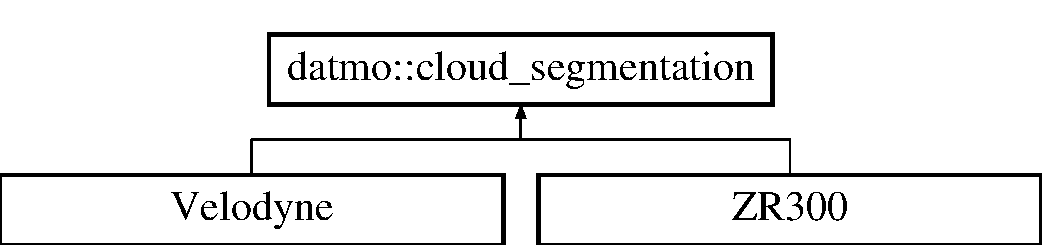
\includegraphics[height=2.000000cm]{classdatmo_1_1cloud__segmentation}
\end{center}
\end{figure}
\subsection*{Public Member Functions}
\begin{DoxyCompactItemize}
\item 
\hyperlink{classdatmo_1_1cloud__segmentation_a7624176c1ff33d2fa3930bf9eef89c19}{cloud\+\_\+segmentation} ()
\item 
\hyperlink{classdatmo_1_1cloud__segmentation_a493c03c6c372488ed9b507b296af2ed4}{$\sim$cloud\+\_\+segmentation} ()
\item 
void \hyperlink{classdatmo_1_1cloud__segmentation_a9ad8d99df49f5b55a920d477c4dcc0ef}{init} (ros\+::\+Node\+Handle \&nh, ros\+::\+Node\+Handle \&private\+\_\+nh)
\end{DoxyCompactItemize}
\subsection*{Protected Attributes}
\begin{DoxyCompactItemize}
\item 
ros\+::\+Publisher \hyperlink{classdatmo_1_1cloud__segmentation_a01955e35ed0d12b9da4d4d9afb1007e3}{pub}
\begin{DoxyCompactList}\small\item\em publish point cloud after transforming it to base\+\_\+link on topic /transformed\+\_\+points \end{DoxyCompactList}\item 
ros\+::\+Publisher \hyperlink{classdatmo_1_1cloud__segmentation_a0e1bf18752add68fc2df89e212750d91}{pub\+\_\+2}
\begin{DoxyCompactList}\small\item\em Publish pointcloud with dynamic obstacles on topic /dynamic\+\_\+points. \end{DoxyCompactList}\item 
ros\+::\+Publisher \hyperlink{classdatmo_1_1cloud__segmentation_ac80cc51227bec21bcac68f80a9b4fc47}{pub\+\_\+3}
\begin{DoxyCompactList}\small\item\em Publish pointcloud with dynamic obstacles on topic /dynamic\+\_\+points. \end{DoxyCompactList}\item 
ros\+::\+Publisher \hyperlink{classdatmo_1_1cloud__segmentation_a287579b3989262f060341ebca1ed53b2}{centroids\+\_\+pub}
\begin{DoxyCompactList}\small\item\em Publish geometry\+\_\+msgs\+::\+Pose\+Array centroids of dynamic obstacles on topic /object\+\_\+centroids. \end{DoxyCompactList}\item 
ros\+::\+Subscriber \hyperlink{classdatmo_1_1cloud__segmentation_a72e340852b66e150cb7f0e25214b7439}{sub}
\begin{DoxyCompactList}\small\item\em subscribes sensor\+\_\+msgs\+::\+Point\+Cloud2 from topic /cloud \end{DoxyCompactList}\item 
tf\+::\+Transform\+Listener \hyperlink{classdatmo_1_1cloud__segmentation_abf9b807df25f63ea330b165a9f2e4be1}{listener}
\begin{DoxyCompactList}\small\item\em A TF listener. \end{DoxyCompactList}\item 
tf\+::\+Transform\+Broadcaster \hyperlink{classdatmo_1_1cloud__segmentation_aa2712034cbe68df4d19b0fcf87f9b465}{br}
\begin{DoxyCompactList}\small\item\em TF brodcaster to broadcast relative transfom between current pointcloud and prev Point\+Cloud. \end{DoxyCompactList}\item 
tf\+::\+Stamped\+Transform \hyperlink{classdatmo_1_1cloud__segmentation_a2c01dc948f63510a421297e7cc6a29e5}{current\+\_\+cloud\+\_\+transform}
\begin{DoxyCompactList}\small\item\em Container to store transform of latest pointcloud wrt /odom. \end{DoxyCompactList}\item 
tf\+::\+Stamped\+Transform \hyperlink{classdatmo_1_1cloud__segmentation_a8ab8642656cda3d94db8d9c2e4613644}{ref\+\_\+cloud\+\_\+transform}
\begin{DoxyCompactList}\small\item\em Container to store transform of reference pointcloud wrt /odom. \end{DoxyCompactList}\item 
tf\+::\+Stamped\+Transform \hyperlink{classdatmo_1_1cloud__segmentation_af664f016cfef835a3cfc303675c0a5ec}{prev\+\_\+cloud\+\_\+transform}
\begin{DoxyCompactList}\small\item\em Container to store transform of previous pointcloud wrt /odom. \end{DoxyCompactList}\item 
pcl\+::\+Point\+Cloud$<$ pcl\+::\+Point\+X\+YZ $>$\+::Ptr \hyperlink{classdatmo_1_1cloud__segmentation_a00e99233257fe5a28a039eef13dbc65b}{cloud\+\_\+transformed}
\begin{DoxyCompactList}\small\item\em container to store current pointcloud after transforming it to /base\+\_\+link frame from /sensor frame \end{DoxyCompactList}\item 
pcl\+::\+Point\+Cloud$<$ pcl\+::\+Point\+X\+YZ $>$\+::Ptr \hyperlink{classdatmo_1_1cloud__segmentation_ad946a48ab59bf9f48338f9ef0702181c}{obj\+\_\+cloud}
\begin{DoxyCompactList}\small\item\em container to store pointcloud having both static and dynamic objects \end{DoxyCompactList}\item 
pcl\+::\+Point\+Cloud$<$ pcl\+::\+Point\+X\+YZ $>$\+::Ptr \hyperlink{classdatmo_1_1cloud__segmentation_a4f4926a401828fc5226665963a2212cf}{ref\+\_\+obj\+\_\+cloud}
\begin{DoxyCompactList}\small\item\em container to store object cloud to be used as reference for comparing with object cloud at current time step for octree based spatial change detection \end{DoxyCompactList}\item 
pcl\+::\+Point\+Cloud$<$ pcl\+::\+Point\+X\+Y\+Z\+R\+GB $>$\+::Ptr \hyperlink{classdatmo_1_1cloud__segmentation_a2f85f1a51b2e90dbce996d90cb3e0155}{occuluded\+\_\+cloud}
\begin{DoxyCompactList}\small\item\em container to store the points at current timestep that are in the areas which were occuluded in reference object cloud. (Green in colour) \end{DoxyCompactList}\item 
pcl\+::\+Point\+Cloud$<$ pcl\+::\+Point\+X\+Y\+Z\+R\+GB $>$\+::Ptr \hyperlink{classdatmo_1_1cloud__segmentation_ac9374ddec382dc6dab33b34542a7b21d}{new\+\_\+discovered\+\_\+cloud}
\begin{DoxyCompactList}\small\item\em Container to store points at current timestep that are in the areas which are newly discovered. (Blue in colour) \end{DoxyCompactList}\item 
pcl\+::\+Point\+Cloud$<$ pcl\+::\+Point\+X\+Y\+Z\+R\+GB $>$\+::Ptr \hyperlink{classdatmo_1_1cloud__segmentation_a57c83961f5b33aa5655c679789f36387}{filtered\+\_\+dynamic\+\_\+cloud}
\begin{DoxyCompactList}\small\item\em Container to store filtered dynamic cloud (Red in colour) = dynamic\+\_\+cloud -\/ occuluded\+\_\+cloud -\/ new\+\_\+discovered\+\_\+cloud. \end{DoxyCompactList}\item 
pcl\+::\+Point\+Cloud$<$ pcl\+::\+Point\+X\+Y\+Z\+R\+GB $>$\+::Ptr \hyperlink{classdatmo_1_1cloud__segmentation_a5d51c3fb6f6206ce1e625bd3536414a0}{classified\+\_\+cloud}
\begin{DoxyCompactList}\small\item\em Container to store final classified cloud = filtered\+\_\+dynamic\+\_\+cloud(\+Red) + occuluded\+\_\+cloud(\+Green) + new\+\_\+discovered\+\_\+cloud(\+Blue) \end{DoxyCompactList}\item 
vector$<$ pcl\+::\+Point\+Cloud$<$ pcl\+::\+Point\+X\+YZ $>$\+::Ptr, Eigen\+::aligned\+\_\+allocator$<$ pcl\+::\+Point\+Cloud$<$ pcl\+::\+Point\+X\+YZ $>$\+::Ptr $>$ $>$ \hyperlink{classdatmo_1_1cloud__segmentation_abcf359aaf4f17128e961473692d9c473}{source\+Clouds}
\begin{DoxyCompactList}\small\item\em vector to store the \char`\"{}\+O\+C\+T\+R\+E\+E\+\_\+\+W\+I\+N\+D\+O\+W\char`\"{} number of obj\+\_\+cloud in the memory \end{DoxyCompactList}\item 
vector$<$ tf\+::\+Stamped\+Transform $>$ \hyperlink{classdatmo_1_1cloud__segmentation_a24a81e37b2eff06482f65b09e39af9e4}{source\+Transforms}
\begin{DoxyCompactList}\small\item\em Vector to store corresponding Transforms of each Point\+Cloud in source\+Clouds /odom to /base\+\_\+link. \end{DoxyCompactList}\item 
Eigen\+::\+Affine3d \hyperlink{classdatmo_1_1cloud__segmentation_a9f47c2e7cba42121779e2772a052f58b}{odom\+\_\+transform\+\_\+matrix}
\begin{DoxyCompactList}\small\item\em Container to store relative transform between obj\+\_\+cloud and ref\+\_\+obj\+\_\+cloud. \end{DoxyCompactList}\item 
Eigen\+::\+Affine3f \hyperlink{classdatmo_1_1cloud__segmentation_ac7762960a72df80afdf8bedd59335ddc}{icp\+\_\+transform\+\_\+matrix}
\item 
int \hyperlink{classdatmo_1_1cloud__segmentation_a56499171fe846acfb2a73a5134261a91}{counter}
\item 
string \hyperlink{classdatmo_1_1cloud__segmentation_a16ce63fc6e22bab22c377d9049923119}{frame\+\_\+id}
\item 
string \hyperlink{classdatmo_1_1cloud__segmentation_a744619077c95172db4c19f45dcd9f30c}{base\+\_\+frame\+\_\+id}
\item 
string \hyperlink{classdatmo_1_1cloud__segmentation_a53785ef8494de0fd1efed824562f3368}{sensor\+\_\+frame\+\_\+id}
\item 
bool \hyperlink{classdatmo_1_1cloud__segmentation_a71c4d63aacea33f4c1b172e1ff723163}{E\+N\+A\+B\+L\+E\+\_\+\+I\+CP}
\begin{DoxyCompactList}\small\item\em Enable use of I\+CP to better match obj\+\_\+cloud with ref\+\_\+obj\+\_\+cloud \+: Default it is disabled bcoz of bad results. \end{DoxyCompactList}\item 
bool \hyperlink{classdatmo_1_1cloud__segmentation_a03474f362047eb23fbcc53e5ce943148}{E\+N\+A\+B\+L\+E\+\_\+\+G\+R\+O\+U\+N\+D\+\_\+\+R\+E\+M\+O\+V\+AL}
\begin{DoxyCompactList}\small\item\em Enable use of ransac plane fitting to remove ground points \+: Default it is disabled for \hyperlink{classZR300}{Z\+R300} and enabled for \hyperlink{classVelodyne}{Velodyne}. \end{DoxyCompactList}\item 
bool \hyperlink{classdatmo_1_1cloud__segmentation_aa3af9f5d3b0072cba61c14cff25965cb}{E\+N\+A\+B\+L\+E\+\_\+\+V\+O\+X\+E\+L\+I\+SE}
\begin{DoxyCompactList}\small\item\em Enable voxel filter\+: Default it is enable for \hyperlink{classZR300}{Z\+R300} and disabled for \hyperlink{classVelodyne}{Velodyne}. \end{DoxyCompactList}\item 
bool \hyperlink{classdatmo_1_1cloud__segmentation_a5f7ffa75c60af605cc914de7296cddb1}{E\+N\+A\+B\+L\+E\+\_\+\+O\+C\+C\+L\+U\+S\+I\+O\+N\+\_\+\+D\+E\+T\+E\+C\+T\+I\+ON}
\begin{DoxyCompactList}\small\item\em Enable Occlusion detection so as to prevent false dynamic obstacles detection due to shadow \+: Default it is enabled for \hyperlink{classZR300}{Z\+R300} and enabled for \hyperlink{classVelodyne}{Velodyne}. \end{DoxyCompactList}\item 
float \hyperlink{classdatmo_1_1cloud__segmentation_af6f1f8553f2a18176ae84b78ddea07c9}{V\+O\+X\+E\+L\+\_\+\+L\+E\+A\+F\+\_\+\+S\+I\+ZE}
\item 
bool \hyperlink{classdatmo_1_1cloud__segmentation_ae54c11225658974ed8a37a03815aab0e}{E\+N\+A\+B\+L\+E\+\_\+\+S\+OR}
\begin{DoxyCompactList}\small\item\em Enable Statistical Outlier removal filter\+: Default it is enable for \hyperlink{classZR300}{Z\+R300} and disabled for \hyperlink{classVelodyne}{Velodyne}. \end{DoxyCompactList}\item 
float \hyperlink{classdatmo_1_1cloud__segmentation_abb5b1262c14e68886e01e0230c530b07}{S\+O\+R\+\_\+\+M\+E\+A\+N\+\_\+K}
\begin{DoxyCompactList}\small\item\em number of neighbors to analyze for each point \end{DoxyCompactList}\item 
float \hyperlink{classdatmo_1_1cloud__segmentation_ae1c32b9f5741dd7d212f2745f8784de0}{S\+O\+R\+\_\+\+S\+T\+D\+\_\+\+D\+E\+V\+\_\+\+M\+U\+L\+\_\+\+T\+H\+R\+E\+SH}
\begin{DoxyCompactList}\small\item\em distance in multiples of std dev after which point is considered an outlier \end{DoxyCompactList}\item 
float \hyperlink{classdatmo_1_1cloud__segmentation_a503bba212f9c15b767d512771b1559c2}{P\+A\+S\+S\+\_\+\+X\+\_\+\+M\+IN}
\begin{DoxyCompactList}\small\item\em minimum value in x direction \end{DoxyCompactList}\item 
float \hyperlink{classdatmo_1_1cloud__segmentation_a12f8209c6640d67c23cac18b2d8b7964}{P\+A\+S\+S\+\_\+\+X\+\_\+\+M\+AX}
\begin{DoxyCompactList}\small\item\em maximum value in x direction \end{DoxyCompactList}\item 
float \hyperlink{classdatmo_1_1cloud__segmentation_af95645fb925c485f397321d6e07c4574}{P\+A\+S\+S\+\_\+\+Y\+\_\+\+M\+IN}
\begin{DoxyCompactList}\small\item\em minimum value in y direction \end{DoxyCompactList}\item 
float \hyperlink{classdatmo_1_1cloud__segmentation_abacc76df1e25e42d25c1822c2637fa00}{P\+A\+S\+S\+\_\+\+Y\+\_\+\+M\+AX}
\begin{DoxyCompactList}\small\item\em maximum value in y direction \end{DoxyCompactList}\item 
float \hyperlink{classdatmo_1_1cloud__segmentation_acb71ade7e486ad1cafe15c441903f3e0}{P\+A\+S\+S\+\_\+\+Z\+\_\+\+M\+IN}
\begin{DoxyCompactList}\small\item\em minimum value in z direction \end{DoxyCompactList}\item 
float \hyperlink{classdatmo_1_1cloud__segmentation_a05b70936af05654abb9b1924ab593d08}{P\+A\+S\+S\+\_\+\+Z\+\_\+\+M\+AX}
\begin{DoxyCompactList}\small\item\em maximum value in z direction \end{DoxyCompactList}\item 
int \hyperlink{classdatmo_1_1cloud__segmentation_ada1c6bd7f69249c5317cbe95969498e4}{O\+C\+T\+R\+E\+E\+\_\+\+W\+I\+N\+D\+OW}
\begin{DoxyCompactList}\small\item\em This parameter defines that current pointcloud will be compared with \char`\"{}\+O\+C\+T\+R\+E\+E\+\_\+\+W\+I\+N\+D\+O\+W\char`\"{} times previous pointcloud for spatial change detection. \end{DoxyCompactList}\item 
float \hyperlink{classdatmo_1_1cloud__segmentation_aba086f9f8e05f18c02c042c057854a06}{O\+C\+T\+R\+E\+E\+\_\+\+R\+E\+S\+O\+L\+U\+T\+I\+ON}
\begin{DoxyCompactList}\small\item\em smallest dimension of octree leaf node \end{DoxyCompactList}\item 
float \hyperlink{classdatmo_1_1cloud__segmentation_af33add7f3b00fac5be10ffd87eae057f}{S\+E\+G\+\_\+\+C\+L\+U\+S\+T\+E\+R\+\_\+\+T\+O\+L\+E\+R\+A\+N\+CE}
\begin{DoxyCompactList}\small\item\em Maximum distance between two points to be included in same cluster. \end{DoxyCompactList}\item 
int \hyperlink{classdatmo_1_1cloud__segmentation_acf7cfcaf0ab08a2afffcc2b47048bc81}{S\+E\+G\+\_\+\+M\+I\+N\+\_\+\+C\+L\+U\+S\+T\+E\+R\+\_\+\+S\+I\+ZE}
\begin{DoxyCompactList}\small\item\em Minimum number of points that should be present within a cluster. \end{DoxyCompactList}\item 
int \hyperlink{classdatmo_1_1cloud__segmentation_ab2959ad226faeaab4910f42ba91d37cb}{S\+E\+G\+\_\+\+M\+A\+X\+\_\+\+C\+L\+U\+S\+T\+E\+R\+\_\+\+S\+I\+ZE}
\begin{DoxyCompactList}\small\item\em Maximum number points to be included in same cluster. \end{DoxyCompactList}\end{DoxyCompactItemize}
\subsection*{Private Member Functions}
\begin{DoxyCompactItemize}
\item 
void \hyperlink{classdatmo_1_1cloud__segmentation_a9fb8b8321055b7798ce62d1cd9416642}{cloud\+\_\+cb} (const sensor\+\_\+msgs\+::\+Point\+Cloud2\+Const\+Ptr \&cloud\+\_\+msg)
\item 
void \hyperlink{classdatmo_1_1cloud__segmentation_a3e3bd9d1b4a99da4bcd81ebac95f83fe}{cloud\+\_\+transform} (const pcl\+::\+Point\+Cloud$<$ pcl\+::\+Point\+X\+YZ $>$\+::Const\+Ptr \&cloud\+\_\+in, const pcl\+::\+Point\+Cloud$<$ pcl\+::\+Point\+X\+YZ $>$\+::Ptr \&cloud\+\_\+out)
\item 
void \hyperlink{classdatmo_1_1cloud__segmentation_afa29d45018811393b160e64b1f972289}{cloud\+\_\+filter} (const pcl\+::\+Point\+Cloud$<$ pcl\+::\+Point\+X\+YZ $>$\+::Ptr \&cloud\+\_\+in, const string field, float min, float max)
\item 
void \hyperlink{classdatmo_1_1cloud__segmentation_acb0e7e196b28d7d62fe73d7437e629dc}{Voxel\+\_\+filter} (const pcl\+::\+Point\+Cloud$<$ pcl\+::\+Point\+X\+YZ $>$\+::Ptr \&cloud\+\_\+in, const pcl\+::\+Point\+Cloud$<$ pcl\+::\+Point\+X\+YZ $>$\+::Ptr \&cloud\+\_\+out, float \hyperlink{classdatmo_1_1cloud__segmentation_af6f1f8553f2a18176ae84b78ddea07c9}{V\+O\+X\+E\+L\+\_\+\+L\+E\+A\+F\+\_\+\+S\+I\+ZE})
\item 
void \hyperlink{classdatmo_1_1cloud__segmentation_a169ebef33c020301b83261ee2d3f49df}{S\+O\+R\+\_\+filter} (const pcl\+::\+Point\+Cloud$<$ pcl\+::\+Point\+X\+YZ $>$\+::Ptr \&cloud\+\_\+in, const pcl\+::\+Point\+Cloud$<$ pcl\+::\+Point\+X\+YZ $>$\+::Ptr \&cloud\+\_\+out, float \hyperlink{classdatmo_1_1cloud__segmentation_abb5b1262c14e68886e01e0230c530b07}{S\+O\+R\+\_\+\+M\+E\+A\+N\+\_\+K}, float \hyperlink{classdatmo_1_1cloud__segmentation_ae1c32b9f5741dd7d212f2745f8784de0}{S\+O\+R\+\_\+\+S\+T\+D\+\_\+\+D\+E\+V\+\_\+\+M\+U\+L\+\_\+\+T\+H\+R\+E\+SH})
\item 
void \hyperlink{classdatmo_1_1cloud__segmentation_a168514d0652e6ada8a371604470b98ed}{Ransac\+\_\+plane} (const pcl\+::\+Point\+Cloud$<$ pcl\+::\+Point\+X\+YZ $>$\+::Ptr \&cloud\+\_\+in, const pcl\+::\+Point\+Cloud$<$ pcl\+::\+Point\+X\+YZ $>$\+::Ptr \&cloud\+\_\+out)
\item 
void \hyperlink{classdatmo_1_1cloud__segmentation_a7506a589048c71ab56a49d6470591ef1}{euclideancluster} (const pcl\+::\+Point\+Cloud$<$ pcl\+::\+Point\+X\+YZ $>$\+::Ptr \&cloud, float \hyperlink{classdatmo_1_1cloud__segmentation_af33add7f3b00fac5be10ffd87eae057f}{S\+E\+G\+\_\+\+C\+L\+U\+S\+T\+E\+R\+\_\+\+T\+O\+L\+E\+R\+A\+N\+CE}, int \hyperlink{classdatmo_1_1cloud__segmentation_acf7cfcaf0ab08a2afffcc2b47048bc81}{S\+E\+G\+\_\+\+M\+I\+N\+\_\+\+C\+L\+U\+S\+T\+E\+R\+\_\+\+S\+I\+ZE}, int \hyperlink{classdatmo_1_1cloud__segmentation_ab2959ad226faeaab4910f42ba91d37cb}{S\+E\+G\+\_\+\+M\+A\+X\+\_\+\+C\+L\+U\+S\+T\+E\+R\+\_\+\+S\+I\+ZE})
\item 
void \hyperlink{classdatmo_1_1cloud__segmentation_a6dcd90f46e590756a42aafd290443fcf}{detect\+\_\+spatial\+\_\+change} (const pcl\+::\+Point\+Cloud$<$ pcl\+::\+Point\+X\+YZ $>$\+::Ptr \&cloud\+\_\+now, const pcl\+::\+Point\+Cloud$<$ pcl\+::\+Point\+X\+YZ $>$\+::Ptr \&cloud\+\_\+to\+\_\+compare, const pcl\+::\+Point\+Cloud$<$ pcl\+::\+Point\+X\+YZ $>$\+::Ptr \&dynamic\+\_\+cloud, const pcl\+::\+Point\+Cloud$<$ pcl\+::\+Point\+X\+Y\+Z\+R\+GB $>$\+::Ptr \&\hyperlink{classdatmo_1_1cloud__segmentation_a2f85f1a51b2e90dbce996d90cb3e0155}{occuluded\+\_\+cloud}, float \hyperlink{classdatmo_1_1cloud__segmentation_aba086f9f8e05f18c02c042c057854a06}{O\+C\+T\+R\+E\+E\+\_\+\+R\+E\+S\+O\+L\+U\+T\+I\+ON}, bool \hyperlink{classdatmo_1_1cloud__segmentation_a5f7ffa75c60af605cc914de7296cddb1}{E\+N\+A\+B\+L\+E\+\_\+\+O\+C\+C\+L\+U\+S\+I\+O\+N\+\_\+\+D\+E\+T\+E\+C\+T\+I\+ON})
\item 
bool \hyperlink{classdatmo_1_1cloud__segmentation_a5bcf85ac924671c64840ac2087877a5f}{is\+\_\+in\+\_\+bounding\+\_\+area} (const pcl\+::\+Point\+Cloud$<$ pcl\+::\+Point\+X\+YZ $>$\+::Ptr \&coord, pcl\+::\+Point\+X\+Y\+Z\+R\+GB pt)
\item 
void \hyperlink{classdatmo_1_1cloud__segmentation_a2386bd377507c5e1029f73285d8e7251}{integrate\+Odom\+\_\+\+I\+CP} (const pcl\+::\+Point\+Cloud$<$ pcl\+::\+Point\+X\+YZ $>$\+::Const\+Ptr \&\hyperlink{classdatmo_1_1cloud__segmentation_ad946a48ab59bf9f48338f9ef0702181c}{obj\+\_\+cloud}, const pcl\+::\+Point\+Cloud$<$ pcl\+::\+Point\+X\+YZ $>$\+::Ptr \&\hyperlink{classdatmo_1_1cloud__segmentation_a4f4926a401828fc5226665963a2212cf}{ref\+\_\+obj\+\_\+cloud})
\end{DoxyCompactItemize}


\subsection{Constructor \& Destructor Documentation}
\mbox{\Hypertarget{classdatmo_1_1cloud__segmentation_a7624176c1ff33d2fa3930bf9eef89c19}\label{classdatmo_1_1cloud__segmentation_a7624176c1ff33d2fa3930bf9eef89c19}} 
\index{datmo\+::cloud\+\_\+segmentation@{datmo\+::cloud\+\_\+segmentation}!cloud\+\_\+segmentation@{cloud\+\_\+segmentation}}
\index{cloud\+\_\+segmentation@{cloud\+\_\+segmentation}!datmo\+::cloud\+\_\+segmentation@{datmo\+::cloud\+\_\+segmentation}}
\subsubsection{\texorpdfstring{cloud\+\_\+segmentation()}{cloud\_segmentation()}}
{\footnotesize\ttfamily cloud\+\_\+segmentation\+::cloud\+\_\+segmentation (\begin{DoxyParamCaption}{ }\end{DoxyParamCaption})}

\mbox{\Hypertarget{classdatmo_1_1cloud__segmentation_a493c03c6c372488ed9b507b296af2ed4}\label{classdatmo_1_1cloud__segmentation_a493c03c6c372488ed9b507b296af2ed4}} 
\index{datmo\+::cloud\+\_\+segmentation@{datmo\+::cloud\+\_\+segmentation}!````~cloud\+\_\+segmentation@{$\sim$cloud\+\_\+segmentation}}
\index{````~cloud\+\_\+segmentation@{$\sim$cloud\+\_\+segmentation}!datmo\+::cloud\+\_\+segmentation@{datmo\+::cloud\+\_\+segmentation}}
\subsubsection{\texorpdfstring{$\sim$cloud\+\_\+segmentation()}{~cloud\_segmentation()}}
{\footnotesize\ttfamily cloud\+\_\+segmentation\+::$\sim$cloud\+\_\+segmentation (\begin{DoxyParamCaption}{ }\end{DoxyParamCaption})}



\subsection{Member Function Documentation}
\mbox{\Hypertarget{classdatmo_1_1cloud__segmentation_a9fb8b8321055b7798ce62d1cd9416642}\label{classdatmo_1_1cloud__segmentation_a9fb8b8321055b7798ce62d1cd9416642}} 
\index{datmo\+::cloud\+\_\+segmentation@{datmo\+::cloud\+\_\+segmentation}!cloud\+\_\+cb@{cloud\+\_\+cb}}
\index{cloud\+\_\+cb@{cloud\+\_\+cb}!datmo\+::cloud\+\_\+segmentation@{datmo\+::cloud\+\_\+segmentation}}
\subsubsection{\texorpdfstring{cloud\+\_\+cb()}{cloud\_cb()}}
{\footnotesize\ttfamily void cloud\+\_\+segmentation\+::cloud\+\_\+cb (\begin{DoxyParamCaption}\item[{const sensor\+\_\+msgs\+::\+Point\+Cloud2\+Const\+Ptr \&}]{cloud\+\_\+msg }\end{DoxyParamCaption})\hspace{0.3cm}{\ttfamily [private]}}

Callback function get called every time a new point cloud is recieved 
\begin{DoxyParams}[1]{Parameters}
\mbox{\tt in}  & {\em cloud\+\_\+msg} & constant pointer to sensor\+\_\+msgs Point\+Cloud2 \\
\hline
\end{DoxyParams}
\mbox{\Hypertarget{classdatmo_1_1cloud__segmentation_afa29d45018811393b160e64b1f972289}\label{classdatmo_1_1cloud__segmentation_afa29d45018811393b160e64b1f972289}} 
\index{datmo\+::cloud\+\_\+segmentation@{datmo\+::cloud\+\_\+segmentation}!cloud\+\_\+filter@{cloud\+\_\+filter}}
\index{cloud\+\_\+filter@{cloud\+\_\+filter}!datmo\+::cloud\+\_\+segmentation@{datmo\+::cloud\+\_\+segmentation}}
\subsubsection{\texorpdfstring{cloud\+\_\+filter()}{cloud\_filter()}}
{\footnotesize\ttfamily void cloud\+\_\+segmentation\+::cloud\+\_\+filter (\begin{DoxyParamCaption}\item[{const pcl\+::\+Point\+Cloud$<$ pcl\+::\+Point\+X\+YZ $>$\+::Ptr \&}]{cloud\+\_\+in,  }\item[{const string}]{field,  }\item[{float}]{min,  }\item[{float}]{max }\end{DoxyParamCaption})\hspace{0.3cm}{\ttfamily [private]}}

filters the pointcloud wiithin given dimensions and field 
\begin{DoxyParams}[1]{Parameters}
\mbox{\tt in,out}  & {\em cloud\+\_\+in} & ponitcloud to be filtered \\
\hline
\mbox{\tt in}  & {\em field} & axis name (\char`\"{}x\char`\"{} or \char`\"{}y\char`\"{} or \char`\"{}z\char`\"{}) \\
\hline
\mbox{\tt in}  & {\em min} & minimum value of points in given field \\
\hline
\mbox{\tt in}  & {\em max} & maximum value of points in given field \\
\hline
\end{DoxyParams}
\mbox{\Hypertarget{classdatmo_1_1cloud__segmentation_a3e3bd9d1b4a99da4bcd81ebac95f83fe}\label{classdatmo_1_1cloud__segmentation_a3e3bd9d1b4a99da4bcd81ebac95f83fe}} 
\index{datmo\+::cloud\+\_\+segmentation@{datmo\+::cloud\+\_\+segmentation}!cloud\+\_\+transform@{cloud\+\_\+transform}}
\index{cloud\+\_\+transform@{cloud\+\_\+transform}!datmo\+::cloud\+\_\+segmentation@{datmo\+::cloud\+\_\+segmentation}}
\subsubsection{\texorpdfstring{cloud\+\_\+transform()}{cloud\_transform()}}
{\footnotesize\ttfamily void cloud\+\_\+segmentation\+::cloud\+\_\+transform (\begin{DoxyParamCaption}\item[{const pcl\+::\+Point\+Cloud$<$ pcl\+::\+Point\+X\+YZ $>$\+::Const\+Ptr \&}]{cloud\+\_\+in,  }\item[{const pcl\+::\+Point\+Cloud$<$ pcl\+::\+Point\+X\+YZ $>$\+::Ptr \&}]{cloud\+\_\+out }\end{DoxyParamCaption})\hspace{0.3cm}{\ttfamily [private]}}

Transforms the point cloud from sensor\+\_\+frame\+\_\+id to base\+\_\+link This function contains a TF listener 
\begin{DoxyParams}[1]{Parameters}
\mbox{\tt in}  & {\em cloud\+\_\+in} & \\
\hline
\mbox{\tt out}  & {\em cloud\+\_\+out} & \\
\hline
\end{DoxyParams}
\mbox{\Hypertarget{classdatmo_1_1cloud__segmentation_a6dcd90f46e590756a42aafd290443fcf}\label{classdatmo_1_1cloud__segmentation_a6dcd90f46e590756a42aafd290443fcf}} 
\index{datmo\+::cloud\+\_\+segmentation@{datmo\+::cloud\+\_\+segmentation}!detect\+\_\+spatial\+\_\+change@{detect\+\_\+spatial\+\_\+change}}
\index{detect\+\_\+spatial\+\_\+change@{detect\+\_\+spatial\+\_\+change}!datmo\+::cloud\+\_\+segmentation@{datmo\+::cloud\+\_\+segmentation}}
\subsubsection{\texorpdfstring{detect\+\_\+spatial\+\_\+change()}{detect\_spatial\_change()}}
{\footnotesize\ttfamily void cloud\+\_\+segmentation\+::detect\+\_\+spatial\+\_\+change (\begin{DoxyParamCaption}\item[{const pcl\+::\+Point\+Cloud$<$ pcl\+::\+Point\+X\+YZ $>$\+::Ptr \&}]{cloud\+\_\+now,  }\item[{const pcl\+::\+Point\+Cloud$<$ pcl\+::\+Point\+X\+YZ $>$\+::Ptr \&}]{cloud\+\_\+to\+\_\+compare,  }\item[{const pcl\+::\+Point\+Cloud$<$ pcl\+::\+Point\+X\+YZ $>$\+::Ptr \&}]{dynamic\+\_\+cloud,  }\item[{const pcl\+::\+Point\+Cloud$<$ pcl\+::\+Point\+X\+Y\+Z\+R\+GB $>$\+::Ptr \&}]{occuluded\+\_\+cloud,  }\item[{float}]{O\+C\+T\+R\+E\+E\+\_\+\+R\+E\+S\+O\+L\+U\+T\+I\+ON,  }\item[{bool}]{E\+N\+A\+B\+L\+E\+\_\+\+O\+C\+C\+L\+U\+S\+I\+O\+N\+\_\+\+D\+E\+T\+E\+C\+T\+I\+ON }\end{DoxyParamCaption})\hspace{0.3cm}{\ttfamily [private]}}

This function is core for classifying between dynamic and static objects. We used Octree based spatial change detection to find dynamic points more information follow link\+: \href{http://pointclouds.org/documentation/tutorials/octree_change.php}{\tt http\+://pointclouds.\+org/documentation/tutorials/octree\+\_\+change.\+php} We compare the object cloud(obj\+\_\+cloud) at current time step with object cloud \char`\"{}octree\+\_\+window\char`\"{} times previous object cloud (ref\+\_\+obj\+\_\+cloud) We are trying to find the new octree leaf that are created in current obj\+\_\+cloud that were not present previously.

Since the vehicle is moving Previous object cloud first has to be transformed to the frame of object cloud at current time step before pluging into this function

O\+C\+T\+R\+E\+E\+\_\+\+W\+I\+N\+D\+OW and O\+C\+T\+R\+E\+E\+\_\+\+R\+E\+S\+O\+L\+U\+T\+I\+ON parameter can be used for tweaking dynamic object detection For Example\+: \hyperlink{classVelodyne}{Velodyne} data is published at 10 HZ, Keeping O\+C\+T\+R\+E\+E\+\_\+\+W\+I\+N\+D\+OW = 5 and O\+C\+T\+R\+E\+E\+\_\+\+R\+E\+S\+O\+L\+U\+T\+I\+ON = 0.\+4 means that and object would be detected as dynamic if it has moved minimum of 0.\+4m distancein half sec.

zr300 data is published at 30 Hz , Keeping O\+C\+T\+R\+E\+E\+\_\+\+W\+I\+N\+D\+OW = 15 and O\+C\+T\+R\+E\+E\+\_\+\+R\+E\+S\+O\+L\+U\+T\+I\+ON = 0.\+4 means that and object would be detected as dynamic if it has moved minimum of 0.\+4m distancein half sec.


\begin{DoxyParams}{Parameters}
{\em cloud\+\_\+now} & \mbox{[}description\mbox{]} \\
\hline
{\em cloud\+\_\+to\+\_\+compare} & \mbox{[}description\mbox{]} \\
\hline
{\em dynamic\+\_\+cloud} & \mbox{[}description\mbox{]} \\
\hline
{\em occuluded\+\_\+cloud} & \mbox{[}description\mbox{]} \\
\hline
{\em O\+C\+T\+R\+E\+E\+\_\+\+R\+E\+S\+O\+L\+U\+T\+I\+ON} & \mbox{[}description\mbox{]} \\
\hline
{\em E\+N\+A\+B\+L\+E\+\_\+\+O\+C\+C\+L\+U\+S\+I\+O\+N\+\_\+\+D\+E\+T\+E\+C\+T\+I\+ON} & Enables occlusion detection \\
\hline
\end{DoxyParams}
\mbox{\Hypertarget{classdatmo_1_1cloud__segmentation_a7506a589048c71ab56a49d6470591ef1}\label{classdatmo_1_1cloud__segmentation_a7506a589048c71ab56a49d6470591ef1}} 
\index{datmo\+::cloud\+\_\+segmentation@{datmo\+::cloud\+\_\+segmentation}!euclideancluster@{euclideancluster}}
\index{euclideancluster@{euclideancluster}!datmo\+::cloud\+\_\+segmentation@{datmo\+::cloud\+\_\+segmentation}}
\subsubsection{\texorpdfstring{euclideancluster()}{euclideancluster()}}
{\footnotesize\ttfamily void cloud\+\_\+segmentation\+::euclideancluster (\begin{DoxyParamCaption}\item[{const pcl\+::\+Point\+Cloud$<$ pcl\+::\+Point\+X\+YZ $>$\+::Ptr \&}]{cloud,  }\item[{float}]{S\+E\+G\+\_\+\+C\+L\+U\+S\+T\+E\+R\+\_\+\+T\+O\+L\+E\+R\+A\+N\+CE,  }\item[{int}]{S\+E\+G\+\_\+\+M\+I\+N\+\_\+\+C\+L\+U\+S\+T\+E\+R\+\_\+\+S\+I\+ZE,  }\item[{int}]{S\+E\+G\+\_\+\+M\+A\+X\+\_\+\+C\+L\+U\+S\+T\+E\+R\+\_\+\+S\+I\+ZE }\end{DoxyParamCaption})\hspace{0.3cm}{\ttfamily [private]}}

This function uses euclidean clustering algorithm to remove outliers. i.\+e remove random points or very small set of clusters. for more information please follow the link\+:http\+://pointclouds.org/documentation/tutorials/cluster\+\_\+extraction.\+php


\begin{DoxyParams}[1]{Parameters}
\mbox{\tt in,out}  & {\em cloud} & The input Point\+Cloud is replaced by filtered Point\+Cloud \\
\hline
\mbox{\tt in}  & {\em S\+E\+G\+\_\+\+C\+L\+U\+S\+T\+E\+R\+\_\+\+T\+O\+L\+E\+R\+A\+N\+CE} & \\
\hline
\mbox{\tt in}  & {\em S\+E\+G\+\_\+\+M\+I\+N\+\_\+\+C\+L\+U\+S\+T\+E\+R\+\_\+\+S\+I\+ZE} & \\
\hline
\mbox{\tt in}  & {\em S\+E\+G\+\_\+\+M\+A\+X\+\_\+\+C\+L\+U\+S\+T\+E\+R\+\_\+\+S\+I\+ZE} & \\
\hline
\end{DoxyParams}
\mbox{\Hypertarget{classdatmo_1_1cloud__segmentation_a9ad8d99df49f5b55a920d477c4dcc0ef}\label{classdatmo_1_1cloud__segmentation_a9ad8d99df49f5b55a920d477c4dcc0ef}} 
\index{datmo\+::cloud\+\_\+segmentation@{datmo\+::cloud\+\_\+segmentation}!init@{init}}
\index{init@{init}!datmo\+::cloud\+\_\+segmentation@{datmo\+::cloud\+\_\+segmentation}}
\subsubsection{\texorpdfstring{init()}{init()}}
{\footnotesize\ttfamily void cloud\+\_\+segmentation\+::init (\begin{DoxyParamCaption}\item[{ros\+::\+Node\+Handle \&}]{nh,  }\item[{ros\+::\+Node\+Handle \&}]{private\+\_\+nh }\end{DoxyParamCaption})}

\mbox{\Hypertarget{classdatmo_1_1cloud__segmentation_a2386bd377507c5e1029f73285d8e7251}\label{classdatmo_1_1cloud__segmentation_a2386bd377507c5e1029f73285d8e7251}} 
\index{datmo\+::cloud\+\_\+segmentation@{datmo\+::cloud\+\_\+segmentation}!integrate\+Odom\+\_\+\+I\+CP@{integrate\+Odom\+\_\+\+I\+CP}}
\index{integrate\+Odom\+\_\+\+I\+CP@{integrate\+Odom\+\_\+\+I\+CP}!datmo\+::cloud\+\_\+segmentation@{datmo\+::cloud\+\_\+segmentation}}
\subsubsection{\texorpdfstring{integrate\+Odom\+\_\+\+I\+C\+P()}{integrateOdom\_ICP()}}
{\footnotesize\ttfamily void cloud\+\_\+segmentation\+::integrate\+Odom\+\_\+\+I\+CP (\begin{DoxyParamCaption}\item[{const pcl\+::\+Point\+Cloud$<$ pcl\+::\+Point\+X\+YZ $>$\+::Const\+Ptr \&}]{obj\+\_\+cloud,  }\item[{const pcl\+::\+Point\+Cloud$<$ pcl\+::\+Point\+X\+YZ $>$\+::Ptr \&}]{ref\+\_\+obj\+\_\+cloud }\end{DoxyParamCaption})\hspace{0.3cm}{\ttfamily [private]}}

\mbox{\Hypertarget{classdatmo_1_1cloud__segmentation_a5bcf85ac924671c64840ac2087877a5f}\label{classdatmo_1_1cloud__segmentation_a5bcf85ac924671c64840ac2087877a5f}} 
\index{datmo\+::cloud\+\_\+segmentation@{datmo\+::cloud\+\_\+segmentation}!is\+\_\+in\+\_\+bounding\+\_\+area@{is\+\_\+in\+\_\+bounding\+\_\+area}}
\index{is\+\_\+in\+\_\+bounding\+\_\+area@{is\+\_\+in\+\_\+bounding\+\_\+area}!datmo\+::cloud\+\_\+segmentation@{datmo\+::cloud\+\_\+segmentation}}
\subsubsection{\texorpdfstring{is\+\_\+in\+\_\+bounding\+\_\+area()}{is\_in\_bounding\_area()}}
{\footnotesize\ttfamily bool cloud\+\_\+segmentation\+::is\+\_\+in\+\_\+bounding\+\_\+area (\begin{DoxyParamCaption}\item[{const pcl\+::\+Point\+Cloud$<$ pcl\+::\+Point\+X\+YZ $>$\+::Ptr \&}]{coord,  }\item[{pcl\+::\+Point\+X\+Y\+Z\+R\+GB}]{pt }\end{DoxyParamCaption})\hspace{0.3cm}{\ttfamily [private]}}

Since our vehicle is moving we keep exploring new areas. The points those detected in these new areas are classified as dynamic by Spatial change detection algorithm because these points did not existed in previous time step i.\+e in reference cloud.

Lets say coordinates of our bounding area is (P\+A\+S\+S\+\_\+\+X\+\_\+\+M\+IN, P\+A\+S\+S\+\_\+\+Y\+\_\+\+M\+AX) (P\+A\+S\+S\+\_\+\+X\+\_\+\+M\+AX, P\+A\+S\+S\+\_\+\+Y\+\_\+\+M\+AX) (P\+A\+S\+S\+\_\+\+X\+\_\+\+M\+AX, P\+A\+S\+S\+\_\+\+Y\+\_\+\+M\+IN) (P\+A\+S\+S\+\_\+\+X\+\_\+\+M\+IN, P\+A\+S\+S\+\_\+\+Y\+\_\+\+M\+IN) as the vehicle moves forward we tranform this bounding area backwards accoridingly.

Now every point that is detected as dynamic is checked if it lies in the bounding area. If not then it is classified as new detected point.

To check whether the point lies within the polygon a ray casting algorithim is used.

for more information to know about the algorithm follow link\+: \href{http://www.geeksforgeeks.org/how-to-check-if-a-given-point-lies-inside-a-polygon/}{\tt http\+://www.\+geeksforgeeks.\+org/how-\/to-\/check-\/if-\/a-\/given-\/point-\/lies-\/inside-\/a-\/polygon/} 
\begin{DoxyParams}[1]{Parameters}
\mbox{\tt in}  & {\em coord} & Point\+Cloud containing 4 points extreme co-\/ordinates of bounding area. \\
\hline
\mbox{\tt in}  & {\em pt} & point to be checked if it lies within bounding area \\
\hline
\end{DoxyParams}
\begin{DoxyReturn}{Returns}
true/false 
\end{DoxyReturn}
\mbox{\Hypertarget{classdatmo_1_1cloud__segmentation_a168514d0652e6ada8a371604470b98ed}\label{classdatmo_1_1cloud__segmentation_a168514d0652e6ada8a371604470b98ed}} 
\index{datmo\+::cloud\+\_\+segmentation@{datmo\+::cloud\+\_\+segmentation}!Ransac\+\_\+plane@{Ransac\+\_\+plane}}
\index{Ransac\+\_\+plane@{Ransac\+\_\+plane}!datmo\+::cloud\+\_\+segmentation@{datmo\+::cloud\+\_\+segmentation}}
\subsubsection{\texorpdfstring{Ransac\+\_\+plane()}{Ransac\_plane()}}
{\footnotesize\ttfamily void cloud\+\_\+segmentation\+::\+Ransac\+\_\+plane (\begin{DoxyParamCaption}\item[{const pcl\+::\+Point\+Cloud$<$ pcl\+::\+Point\+X\+YZ $>$\+::Ptr \&}]{cloud\+\_\+in,  }\item[{const pcl\+::\+Point\+Cloud$<$ pcl\+::\+Point\+X\+YZ $>$\+::Ptr \&}]{cloud\+\_\+out }\end{DoxyParamCaption})\hspace{0.3cm}{\ttfamily [private]}}

This function uses Ransac plane fitting algorithm to find all the points within a point cloud that support a plane model in our case we aim to find a Ground plane and remove all the points belonging to Ground so that we are only left with points belonging to obstacles. For more information follow link\+: \href{http://pointclouds.org/documentation/tutorials/planar_segmentation.php}{\tt http\+://pointclouds.\+org/documentation/tutorials/planar\+\_\+segmentation.\+php}

In this function we filter out the point cloud above certain height so that the most dominating plane to be fit by Ransac is Ground Plane. Since the we have large number of data points using Ransac to fit all of them would be computationally expensive so we only try fit plane to point in surrounding area of our vehicle here x(0m to 30m) y(-\/15m to 15m) and z(less than 0.\+5m). Accuracy and computational time can be changed by tweaking these parameters.

Also for further reducing computational time we randomly choose 500 points and fit Ransac plane to them only....!

For \hyperlink{classZR300}{Z\+R300} point cloud generated do not contain much points on ground hence Ransac\+\_\+plane fitting is not neccessary. Putting a simple cap on height and neglecting all the point below that suffice our purpose. So Ground plane estimation is disabled by default.

For Pointclouds generated by \hyperlink{classVelodyne}{Velodyne} Lidars significant number of point s fall on ground plane and hence properly removing them is neccessary hence Ground Plane estimation is enabled by default.


\begin{DoxyParams}{Parameters}
{\em cloud\+\_\+in} & Point\+Cloud in which ground plane is to be estimated \\
\hline
{\em cloud\+\_\+out} & Point\+Cloud containing only obstacles (after removing ground points from original Point\+Cloud) \\
\hline
\end{DoxyParams}
distance from ransac plane \mbox{\Hypertarget{classdatmo_1_1cloud__segmentation_a169ebef33c020301b83261ee2d3f49df}\label{classdatmo_1_1cloud__segmentation_a169ebef33c020301b83261ee2d3f49df}} 
\index{datmo\+::cloud\+\_\+segmentation@{datmo\+::cloud\+\_\+segmentation}!S\+O\+R\+\_\+filter@{S\+O\+R\+\_\+filter}}
\index{S\+O\+R\+\_\+filter@{S\+O\+R\+\_\+filter}!datmo\+::cloud\+\_\+segmentation@{datmo\+::cloud\+\_\+segmentation}}
\subsubsection{\texorpdfstring{S\+O\+R\+\_\+filter()}{SOR\_filter()}}
{\footnotesize\ttfamily void cloud\+\_\+segmentation\+::\+S\+O\+R\+\_\+filter (\begin{DoxyParamCaption}\item[{const pcl\+::\+Point\+Cloud$<$ pcl\+::\+Point\+X\+YZ $>$\+::Ptr \&}]{cloud\+\_\+in,  }\item[{const pcl\+::\+Point\+Cloud$<$ pcl\+::\+Point\+X\+YZ $>$\+::Ptr \&}]{cloud\+\_\+out,  }\item[{float}]{S\+O\+R\+\_\+\+M\+E\+A\+N\+\_\+K,  }\item[{float}]{S\+O\+R\+\_\+\+S\+T\+D\+\_\+\+D\+E\+V\+\_\+\+M\+U\+L\+\_\+\+T\+H\+R\+E\+SH }\end{DoxyParamCaption})\hspace{0.3cm}{\ttfamily [private]}}

Statistical\+Outlier\+Removal filter is used to remove sparse points generated due to noise for more information follow the link\+: \href{http://pointclouds.org/documentation/tutorials/statistical_outlier.php}{\tt http\+://pointclouds.\+org/documentation/tutorials/statistical\+\_\+outlier.\+php} S\+OR filter is required for \hyperlink{classZR300}{Z\+R300} pointcloud data and is disables for \hyperlink{classVelodyne}{Velodyne} pointcloud 
\begin{DoxyParams}[1]{Parameters}
\mbox{\tt in}  & {\em cloud\+\_\+in} & \\
\hline
\mbox{\tt out}  & {\em cloud\+\_\+out} & \\
\hline
\mbox{\tt in}  & {\em S\+O\+R\+\_\+\+M\+E\+A\+N\+\_\+K} & \\
\hline
\mbox{\tt in}  & {\em S\+O\+R\+\_\+\+S\+T\+D\+\_\+\+D\+E\+V\+\_\+\+M\+U\+L\+\_\+\+T\+H\+R\+E\+SH} & \\
\hline
\end{DoxyParams}
\mbox{\Hypertarget{classdatmo_1_1cloud__segmentation_acb0e7e196b28d7d62fe73d7437e629dc}\label{classdatmo_1_1cloud__segmentation_acb0e7e196b28d7d62fe73d7437e629dc}} 
\index{datmo\+::cloud\+\_\+segmentation@{datmo\+::cloud\+\_\+segmentation}!Voxel\+\_\+filter@{Voxel\+\_\+filter}}
\index{Voxel\+\_\+filter@{Voxel\+\_\+filter}!datmo\+::cloud\+\_\+segmentation@{datmo\+::cloud\+\_\+segmentation}}
\subsubsection{\texorpdfstring{Voxel\+\_\+filter()}{Voxel\_filter()}}
{\footnotesize\ttfamily void cloud\+\_\+segmentation\+::\+Voxel\+\_\+filter (\begin{DoxyParamCaption}\item[{const pcl\+::\+Point\+Cloud$<$ pcl\+::\+Point\+X\+YZ $>$\+::Ptr \&}]{cloud\+\_\+in,  }\item[{const pcl\+::\+Point\+Cloud$<$ pcl\+::\+Point\+X\+YZ $>$\+::Ptr \&}]{cloud\+\_\+out,  }\item[{float}]{V\+O\+X\+E\+L\+\_\+\+L\+E\+A\+F\+\_\+\+S\+I\+ZE }\end{DoxyParamCaption})\hspace{0.3cm}{\ttfamily [private]}}

This function downsamples a Point\+Cloud that is, reduce the number of points – a point cloud dataset, using a voxelized grid approach For more information follow the link \href{http://pointclouds.org/documentation/tutorials/voxel_grid.php}{\tt http\+://pointclouds.\+org/documentation/tutorials/voxel\+\_\+grid.\+php} Also it removes any nan values in pointcloud This filter is neccessary for the dense Point\+Cloud generated by stereo camera like Z\+ED stereo camera and R\+G\+BD camera like \hyperlink{classZR300}{Z\+R300} Point\+Cloud generated by 3D Lidars like \hyperlink{classVelodyne}{Velodyne} and Quanergy are very sparse and hence is disable for them by default. 
\begin{DoxyParams}[1]{Parameters}
\mbox{\tt in}  & {\em cloud\+\_\+in} & \\
\hline
\mbox{\tt out}  & {\em cloud\+\_\+out} & \\
\hline
\mbox{\tt in}  & {\em V\+O\+X\+E\+L\+\_\+\+L\+E\+A\+F\+\_\+\+S\+I\+ZE} & \\
\hline
\end{DoxyParams}


\subsection{Member Data Documentation}
\mbox{\Hypertarget{classdatmo_1_1cloud__segmentation_a744619077c95172db4c19f45dcd9f30c}\label{classdatmo_1_1cloud__segmentation_a744619077c95172db4c19f45dcd9f30c}} 
\index{datmo\+::cloud\+\_\+segmentation@{datmo\+::cloud\+\_\+segmentation}!base\+\_\+frame\+\_\+id@{base\+\_\+frame\+\_\+id}}
\index{base\+\_\+frame\+\_\+id@{base\+\_\+frame\+\_\+id}!datmo\+::cloud\+\_\+segmentation@{datmo\+::cloud\+\_\+segmentation}}
\subsubsection{\texorpdfstring{base\+\_\+frame\+\_\+id}{base\_frame\_id}}
{\footnotesize\ttfamily string datmo\+::cloud\+\_\+segmentation\+::base\+\_\+frame\+\_\+id\hspace{0.3cm}{\ttfamily [protected]}}

\mbox{\Hypertarget{classdatmo_1_1cloud__segmentation_aa2712034cbe68df4d19b0fcf87f9b465}\label{classdatmo_1_1cloud__segmentation_aa2712034cbe68df4d19b0fcf87f9b465}} 
\index{datmo\+::cloud\+\_\+segmentation@{datmo\+::cloud\+\_\+segmentation}!br@{br}}
\index{br@{br}!datmo\+::cloud\+\_\+segmentation@{datmo\+::cloud\+\_\+segmentation}}
\subsubsection{\texorpdfstring{br}{br}}
{\footnotesize\ttfamily tf\+::\+Transform\+Broadcaster datmo\+::cloud\+\_\+segmentation\+::br\hspace{0.3cm}{\ttfamily [protected]}}



TF brodcaster to broadcast relative transfom between current pointcloud and prev Point\+Cloud. 

\mbox{\Hypertarget{classdatmo_1_1cloud__segmentation_a287579b3989262f060341ebca1ed53b2}\label{classdatmo_1_1cloud__segmentation_a287579b3989262f060341ebca1ed53b2}} 
\index{datmo\+::cloud\+\_\+segmentation@{datmo\+::cloud\+\_\+segmentation}!centroids\+\_\+pub@{centroids\+\_\+pub}}
\index{centroids\+\_\+pub@{centroids\+\_\+pub}!datmo\+::cloud\+\_\+segmentation@{datmo\+::cloud\+\_\+segmentation}}
\subsubsection{\texorpdfstring{centroids\+\_\+pub}{centroids\_pub}}
{\footnotesize\ttfamily ros\+::\+Publisher datmo\+::cloud\+\_\+segmentation\+::centroids\+\_\+pub\hspace{0.3cm}{\ttfamily [protected]}}



Publish geometry\+\_\+msgs\+::\+Pose\+Array centroids of dynamic obstacles on topic /object\+\_\+centroids. 

\mbox{\Hypertarget{classdatmo_1_1cloud__segmentation_a5d51c3fb6f6206ce1e625bd3536414a0}\label{classdatmo_1_1cloud__segmentation_a5d51c3fb6f6206ce1e625bd3536414a0}} 
\index{datmo\+::cloud\+\_\+segmentation@{datmo\+::cloud\+\_\+segmentation}!classified\+\_\+cloud@{classified\+\_\+cloud}}
\index{classified\+\_\+cloud@{classified\+\_\+cloud}!datmo\+::cloud\+\_\+segmentation@{datmo\+::cloud\+\_\+segmentation}}
\subsubsection{\texorpdfstring{classified\+\_\+cloud}{classified\_cloud}}
{\footnotesize\ttfamily pcl\+::\+Point\+Cloud$<$pcl\+::\+Point\+X\+Y\+Z\+R\+GB$>$\+::Ptr datmo\+::cloud\+\_\+segmentation\+::classified\+\_\+cloud\hspace{0.3cm}{\ttfamily [protected]}}



Container to store final classified cloud = filtered\+\_\+dynamic\+\_\+cloud(\+Red) + occuluded\+\_\+cloud(\+Green) + new\+\_\+discovered\+\_\+cloud(\+Blue) 

\mbox{\Hypertarget{classdatmo_1_1cloud__segmentation_a00e99233257fe5a28a039eef13dbc65b}\label{classdatmo_1_1cloud__segmentation_a00e99233257fe5a28a039eef13dbc65b}} 
\index{datmo\+::cloud\+\_\+segmentation@{datmo\+::cloud\+\_\+segmentation}!cloud\+\_\+transformed@{cloud\+\_\+transformed}}
\index{cloud\+\_\+transformed@{cloud\+\_\+transformed}!datmo\+::cloud\+\_\+segmentation@{datmo\+::cloud\+\_\+segmentation}}
\subsubsection{\texorpdfstring{cloud\+\_\+transformed}{cloud\_transformed}}
{\footnotesize\ttfamily pcl\+::\+Point\+Cloud$<$pcl\+::\+Point\+X\+YZ$>$\+:: Ptr datmo\+::cloud\+\_\+segmentation\+::cloud\+\_\+transformed\hspace{0.3cm}{\ttfamily [protected]}}



container to store current pointcloud after transforming it to /base\+\_\+link frame from /sensor frame 

\mbox{\Hypertarget{classdatmo_1_1cloud__segmentation_a56499171fe846acfb2a73a5134261a91}\label{classdatmo_1_1cloud__segmentation_a56499171fe846acfb2a73a5134261a91}} 
\index{datmo\+::cloud\+\_\+segmentation@{datmo\+::cloud\+\_\+segmentation}!counter@{counter}}
\index{counter@{counter}!datmo\+::cloud\+\_\+segmentation@{datmo\+::cloud\+\_\+segmentation}}
\subsubsection{\texorpdfstring{counter}{counter}}
{\footnotesize\ttfamily int datmo\+::cloud\+\_\+segmentation\+::counter\hspace{0.3cm}{\ttfamily [protected]}}

\mbox{\Hypertarget{classdatmo_1_1cloud__segmentation_a2c01dc948f63510a421297e7cc6a29e5}\label{classdatmo_1_1cloud__segmentation_a2c01dc948f63510a421297e7cc6a29e5}} 
\index{datmo\+::cloud\+\_\+segmentation@{datmo\+::cloud\+\_\+segmentation}!current\+\_\+cloud\+\_\+transform@{current\+\_\+cloud\+\_\+transform}}
\index{current\+\_\+cloud\+\_\+transform@{current\+\_\+cloud\+\_\+transform}!datmo\+::cloud\+\_\+segmentation@{datmo\+::cloud\+\_\+segmentation}}
\subsubsection{\texorpdfstring{current\+\_\+cloud\+\_\+transform}{current\_cloud\_transform}}
{\footnotesize\ttfamily tf\+::\+Stamped\+Transform datmo\+::cloud\+\_\+segmentation\+::current\+\_\+cloud\+\_\+transform\hspace{0.3cm}{\ttfamily [protected]}}



Container to store transform of latest pointcloud wrt /odom. 

\mbox{\Hypertarget{classdatmo_1_1cloud__segmentation_a03474f362047eb23fbcc53e5ce943148}\label{classdatmo_1_1cloud__segmentation_a03474f362047eb23fbcc53e5ce943148}} 
\index{datmo\+::cloud\+\_\+segmentation@{datmo\+::cloud\+\_\+segmentation}!E\+N\+A\+B\+L\+E\+\_\+\+G\+R\+O\+U\+N\+D\+\_\+\+R\+E\+M\+O\+V\+AL@{E\+N\+A\+B\+L\+E\+\_\+\+G\+R\+O\+U\+N\+D\+\_\+\+R\+E\+M\+O\+V\+AL}}
\index{E\+N\+A\+B\+L\+E\+\_\+\+G\+R\+O\+U\+N\+D\+\_\+\+R\+E\+M\+O\+V\+AL@{E\+N\+A\+B\+L\+E\+\_\+\+G\+R\+O\+U\+N\+D\+\_\+\+R\+E\+M\+O\+V\+AL}!datmo\+::cloud\+\_\+segmentation@{datmo\+::cloud\+\_\+segmentation}}
\subsubsection{\texorpdfstring{E\+N\+A\+B\+L\+E\+\_\+\+G\+R\+O\+U\+N\+D\+\_\+\+R\+E\+M\+O\+V\+AL}{ENABLE\_GROUND\_REMOVAL}}
{\footnotesize\ttfamily bool datmo\+::cloud\+\_\+segmentation\+::\+E\+N\+A\+B\+L\+E\+\_\+\+G\+R\+O\+U\+N\+D\+\_\+\+R\+E\+M\+O\+V\+AL\hspace{0.3cm}{\ttfamily [protected]}}



Enable use of ransac plane fitting to remove ground points \+: Default it is disabled for \hyperlink{classZR300}{Z\+R300} and enabled for \hyperlink{classVelodyne}{Velodyne}. 

\mbox{\Hypertarget{classdatmo_1_1cloud__segmentation_a71c4d63aacea33f4c1b172e1ff723163}\label{classdatmo_1_1cloud__segmentation_a71c4d63aacea33f4c1b172e1ff723163}} 
\index{datmo\+::cloud\+\_\+segmentation@{datmo\+::cloud\+\_\+segmentation}!E\+N\+A\+B\+L\+E\+\_\+\+I\+CP@{E\+N\+A\+B\+L\+E\+\_\+\+I\+CP}}
\index{E\+N\+A\+B\+L\+E\+\_\+\+I\+CP@{E\+N\+A\+B\+L\+E\+\_\+\+I\+CP}!datmo\+::cloud\+\_\+segmentation@{datmo\+::cloud\+\_\+segmentation}}
\subsubsection{\texorpdfstring{E\+N\+A\+B\+L\+E\+\_\+\+I\+CP}{ENABLE\_ICP}}
{\footnotesize\ttfamily bool datmo\+::cloud\+\_\+segmentation\+::\+E\+N\+A\+B\+L\+E\+\_\+\+I\+CP\hspace{0.3cm}{\ttfamily [protected]}}



Enable use of I\+CP to better match obj\+\_\+cloud with ref\+\_\+obj\+\_\+cloud \+: Default it is disabled bcoz of bad results. 

\mbox{\Hypertarget{classdatmo_1_1cloud__segmentation_a5f7ffa75c60af605cc914de7296cddb1}\label{classdatmo_1_1cloud__segmentation_a5f7ffa75c60af605cc914de7296cddb1}} 
\index{datmo\+::cloud\+\_\+segmentation@{datmo\+::cloud\+\_\+segmentation}!E\+N\+A\+B\+L\+E\+\_\+\+O\+C\+C\+L\+U\+S\+I\+O\+N\+\_\+\+D\+E\+T\+E\+C\+T\+I\+ON@{E\+N\+A\+B\+L\+E\+\_\+\+O\+C\+C\+L\+U\+S\+I\+O\+N\+\_\+\+D\+E\+T\+E\+C\+T\+I\+ON}}
\index{E\+N\+A\+B\+L\+E\+\_\+\+O\+C\+C\+L\+U\+S\+I\+O\+N\+\_\+\+D\+E\+T\+E\+C\+T\+I\+ON@{E\+N\+A\+B\+L\+E\+\_\+\+O\+C\+C\+L\+U\+S\+I\+O\+N\+\_\+\+D\+E\+T\+E\+C\+T\+I\+ON}!datmo\+::cloud\+\_\+segmentation@{datmo\+::cloud\+\_\+segmentation}}
\subsubsection{\texorpdfstring{E\+N\+A\+B\+L\+E\+\_\+\+O\+C\+C\+L\+U\+S\+I\+O\+N\+\_\+\+D\+E\+T\+E\+C\+T\+I\+ON}{ENABLE\_OCCLUSION\_DETECTION}}
{\footnotesize\ttfamily bool datmo\+::cloud\+\_\+segmentation\+::\+E\+N\+A\+B\+L\+E\+\_\+\+O\+C\+C\+L\+U\+S\+I\+O\+N\+\_\+\+D\+E\+T\+E\+C\+T\+I\+ON\hspace{0.3cm}{\ttfamily [protected]}}



Enable Occlusion detection so as to prevent false dynamic obstacles detection due to shadow \+: Default it is enabled for \hyperlink{classZR300}{Z\+R300} and enabled for \hyperlink{classVelodyne}{Velodyne}. 

\mbox{\Hypertarget{classdatmo_1_1cloud__segmentation_ae54c11225658974ed8a37a03815aab0e}\label{classdatmo_1_1cloud__segmentation_ae54c11225658974ed8a37a03815aab0e}} 
\index{datmo\+::cloud\+\_\+segmentation@{datmo\+::cloud\+\_\+segmentation}!E\+N\+A\+B\+L\+E\+\_\+\+S\+OR@{E\+N\+A\+B\+L\+E\+\_\+\+S\+OR}}
\index{E\+N\+A\+B\+L\+E\+\_\+\+S\+OR@{E\+N\+A\+B\+L\+E\+\_\+\+S\+OR}!datmo\+::cloud\+\_\+segmentation@{datmo\+::cloud\+\_\+segmentation}}
\subsubsection{\texorpdfstring{E\+N\+A\+B\+L\+E\+\_\+\+S\+OR}{ENABLE\_SOR}}
{\footnotesize\ttfamily bool datmo\+::cloud\+\_\+segmentation\+::\+E\+N\+A\+B\+L\+E\+\_\+\+S\+OR\hspace{0.3cm}{\ttfamily [protected]}}



Enable Statistical Outlier removal filter\+: Default it is enable for \hyperlink{classZR300}{Z\+R300} and disabled for \hyperlink{classVelodyne}{Velodyne}. 

\mbox{\Hypertarget{classdatmo_1_1cloud__segmentation_aa3af9f5d3b0072cba61c14cff25965cb}\label{classdatmo_1_1cloud__segmentation_aa3af9f5d3b0072cba61c14cff25965cb}} 
\index{datmo\+::cloud\+\_\+segmentation@{datmo\+::cloud\+\_\+segmentation}!E\+N\+A\+B\+L\+E\+\_\+\+V\+O\+X\+E\+L\+I\+SE@{E\+N\+A\+B\+L\+E\+\_\+\+V\+O\+X\+E\+L\+I\+SE}}
\index{E\+N\+A\+B\+L\+E\+\_\+\+V\+O\+X\+E\+L\+I\+SE@{E\+N\+A\+B\+L\+E\+\_\+\+V\+O\+X\+E\+L\+I\+SE}!datmo\+::cloud\+\_\+segmentation@{datmo\+::cloud\+\_\+segmentation}}
\subsubsection{\texorpdfstring{E\+N\+A\+B\+L\+E\+\_\+\+V\+O\+X\+E\+L\+I\+SE}{ENABLE\_VOXELISE}}
{\footnotesize\ttfamily bool datmo\+::cloud\+\_\+segmentation\+::\+E\+N\+A\+B\+L\+E\+\_\+\+V\+O\+X\+E\+L\+I\+SE\hspace{0.3cm}{\ttfamily [protected]}}



Enable voxel filter\+: Default it is enable for \hyperlink{classZR300}{Z\+R300} and disabled for \hyperlink{classVelodyne}{Velodyne}. 

\mbox{\Hypertarget{classdatmo_1_1cloud__segmentation_a57c83961f5b33aa5655c679789f36387}\label{classdatmo_1_1cloud__segmentation_a57c83961f5b33aa5655c679789f36387}} 
\index{datmo\+::cloud\+\_\+segmentation@{datmo\+::cloud\+\_\+segmentation}!filtered\+\_\+dynamic\+\_\+cloud@{filtered\+\_\+dynamic\+\_\+cloud}}
\index{filtered\+\_\+dynamic\+\_\+cloud@{filtered\+\_\+dynamic\+\_\+cloud}!datmo\+::cloud\+\_\+segmentation@{datmo\+::cloud\+\_\+segmentation}}
\subsubsection{\texorpdfstring{filtered\+\_\+dynamic\+\_\+cloud}{filtered\_dynamic\_cloud}}
{\footnotesize\ttfamily pcl\+::\+Point\+Cloud$<$pcl\+::\+Point\+X\+Y\+Z\+R\+GB$>$\+::Ptr datmo\+::cloud\+\_\+segmentation\+::filtered\+\_\+dynamic\+\_\+cloud\hspace{0.3cm}{\ttfamily [protected]}}



Container to store filtered dynamic cloud (Red in colour) = dynamic\+\_\+cloud -\/ occuluded\+\_\+cloud -\/ new\+\_\+discovered\+\_\+cloud. 

\mbox{\Hypertarget{classdatmo_1_1cloud__segmentation_a16ce63fc6e22bab22c377d9049923119}\label{classdatmo_1_1cloud__segmentation_a16ce63fc6e22bab22c377d9049923119}} 
\index{datmo\+::cloud\+\_\+segmentation@{datmo\+::cloud\+\_\+segmentation}!frame\+\_\+id@{frame\+\_\+id}}
\index{frame\+\_\+id@{frame\+\_\+id}!datmo\+::cloud\+\_\+segmentation@{datmo\+::cloud\+\_\+segmentation}}
\subsubsection{\texorpdfstring{frame\+\_\+id}{frame\_id}}
{\footnotesize\ttfamily string datmo\+::cloud\+\_\+segmentation\+::frame\+\_\+id\hspace{0.3cm}{\ttfamily [protected]}}

\mbox{\Hypertarget{classdatmo_1_1cloud__segmentation_ac7762960a72df80afdf8bedd59335ddc}\label{classdatmo_1_1cloud__segmentation_ac7762960a72df80afdf8bedd59335ddc}} 
\index{datmo\+::cloud\+\_\+segmentation@{datmo\+::cloud\+\_\+segmentation}!icp\+\_\+transform\+\_\+matrix@{icp\+\_\+transform\+\_\+matrix}}
\index{icp\+\_\+transform\+\_\+matrix@{icp\+\_\+transform\+\_\+matrix}!datmo\+::cloud\+\_\+segmentation@{datmo\+::cloud\+\_\+segmentation}}
\subsubsection{\texorpdfstring{icp\+\_\+transform\+\_\+matrix}{icp\_transform\_matrix}}
{\footnotesize\ttfamily Eigen\+::\+Affine3f datmo\+::cloud\+\_\+segmentation\+::icp\+\_\+transform\+\_\+matrix\hspace{0.3cm}{\ttfamily [protected]}}

\mbox{\Hypertarget{classdatmo_1_1cloud__segmentation_abf9b807df25f63ea330b165a9f2e4be1}\label{classdatmo_1_1cloud__segmentation_abf9b807df25f63ea330b165a9f2e4be1}} 
\index{datmo\+::cloud\+\_\+segmentation@{datmo\+::cloud\+\_\+segmentation}!listener@{listener}}
\index{listener@{listener}!datmo\+::cloud\+\_\+segmentation@{datmo\+::cloud\+\_\+segmentation}}
\subsubsection{\texorpdfstring{listener}{listener}}
{\footnotesize\ttfamily tf\+::\+Transform\+Listener datmo\+::cloud\+\_\+segmentation\+::listener\hspace{0.3cm}{\ttfamily [protected]}}



A TF listener. 

\mbox{\Hypertarget{classdatmo_1_1cloud__segmentation_ac9374ddec382dc6dab33b34542a7b21d}\label{classdatmo_1_1cloud__segmentation_ac9374ddec382dc6dab33b34542a7b21d}} 
\index{datmo\+::cloud\+\_\+segmentation@{datmo\+::cloud\+\_\+segmentation}!new\+\_\+discovered\+\_\+cloud@{new\+\_\+discovered\+\_\+cloud}}
\index{new\+\_\+discovered\+\_\+cloud@{new\+\_\+discovered\+\_\+cloud}!datmo\+::cloud\+\_\+segmentation@{datmo\+::cloud\+\_\+segmentation}}
\subsubsection{\texorpdfstring{new\+\_\+discovered\+\_\+cloud}{new\_discovered\_cloud}}
{\footnotesize\ttfamily pcl\+::\+Point\+Cloud$<$pcl\+::\+Point\+X\+Y\+Z\+R\+GB$>$\+::Ptr datmo\+::cloud\+\_\+segmentation\+::new\+\_\+discovered\+\_\+cloud\hspace{0.3cm}{\ttfamily [protected]}}



Container to store points at current timestep that are in the areas which are newly discovered. (Blue in colour) 

\mbox{\Hypertarget{classdatmo_1_1cloud__segmentation_ad946a48ab59bf9f48338f9ef0702181c}\label{classdatmo_1_1cloud__segmentation_ad946a48ab59bf9f48338f9ef0702181c}} 
\index{datmo\+::cloud\+\_\+segmentation@{datmo\+::cloud\+\_\+segmentation}!obj\+\_\+cloud@{obj\+\_\+cloud}}
\index{obj\+\_\+cloud@{obj\+\_\+cloud}!datmo\+::cloud\+\_\+segmentation@{datmo\+::cloud\+\_\+segmentation}}
\subsubsection{\texorpdfstring{obj\+\_\+cloud}{obj\_cloud}}
{\footnotesize\ttfamily pcl\+::\+Point\+Cloud$<$pcl\+::\+Point\+X\+YZ$>$\+::Ptr datmo\+::cloud\+\_\+segmentation\+::obj\+\_\+cloud\hspace{0.3cm}{\ttfamily [protected]}}



container to store pointcloud having both static and dynamic objects 

\mbox{\Hypertarget{classdatmo_1_1cloud__segmentation_a2f85f1a51b2e90dbce996d90cb3e0155}\label{classdatmo_1_1cloud__segmentation_a2f85f1a51b2e90dbce996d90cb3e0155}} 
\index{datmo\+::cloud\+\_\+segmentation@{datmo\+::cloud\+\_\+segmentation}!occuluded\+\_\+cloud@{occuluded\+\_\+cloud}}
\index{occuluded\+\_\+cloud@{occuluded\+\_\+cloud}!datmo\+::cloud\+\_\+segmentation@{datmo\+::cloud\+\_\+segmentation}}
\subsubsection{\texorpdfstring{occuluded\+\_\+cloud}{occuluded\_cloud}}
{\footnotesize\ttfamily pcl\+::\+Point\+Cloud$<$pcl\+::\+Point\+X\+Y\+Z\+R\+GB$>$\+::Ptr datmo\+::cloud\+\_\+segmentation\+::occuluded\+\_\+cloud\hspace{0.3cm}{\ttfamily [protected]}}



container to store the points at current timestep that are in the areas which were occuluded in reference object cloud. (Green in colour) 

\mbox{\Hypertarget{classdatmo_1_1cloud__segmentation_aba086f9f8e05f18c02c042c057854a06}\label{classdatmo_1_1cloud__segmentation_aba086f9f8e05f18c02c042c057854a06}} 
\index{datmo\+::cloud\+\_\+segmentation@{datmo\+::cloud\+\_\+segmentation}!O\+C\+T\+R\+E\+E\+\_\+\+R\+E\+S\+O\+L\+U\+T\+I\+ON@{O\+C\+T\+R\+E\+E\+\_\+\+R\+E\+S\+O\+L\+U\+T\+I\+ON}}
\index{O\+C\+T\+R\+E\+E\+\_\+\+R\+E\+S\+O\+L\+U\+T\+I\+ON@{O\+C\+T\+R\+E\+E\+\_\+\+R\+E\+S\+O\+L\+U\+T\+I\+ON}!datmo\+::cloud\+\_\+segmentation@{datmo\+::cloud\+\_\+segmentation}}
\subsubsection{\texorpdfstring{O\+C\+T\+R\+E\+E\+\_\+\+R\+E\+S\+O\+L\+U\+T\+I\+ON}{OCTREE\_RESOLUTION}}
{\footnotesize\ttfamily float datmo\+::cloud\+\_\+segmentation\+::\+O\+C\+T\+R\+E\+E\+\_\+\+R\+E\+S\+O\+L\+U\+T\+I\+ON\hspace{0.3cm}{\ttfamily [protected]}}



smallest dimension of octree leaf node 

\mbox{\Hypertarget{classdatmo_1_1cloud__segmentation_ada1c6bd7f69249c5317cbe95969498e4}\label{classdatmo_1_1cloud__segmentation_ada1c6bd7f69249c5317cbe95969498e4}} 
\index{datmo\+::cloud\+\_\+segmentation@{datmo\+::cloud\+\_\+segmentation}!O\+C\+T\+R\+E\+E\+\_\+\+W\+I\+N\+D\+OW@{O\+C\+T\+R\+E\+E\+\_\+\+W\+I\+N\+D\+OW}}
\index{O\+C\+T\+R\+E\+E\+\_\+\+W\+I\+N\+D\+OW@{O\+C\+T\+R\+E\+E\+\_\+\+W\+I\+N\+D\+OW}!datmo\+::cloud\+\_\+segmentation@{datmo\+::cloud\+\_\+segmentation}}
\subsubsection{\texorpdfstring{O\+C\+T\+R\+E\+E\+\_\+\+W\+I\+N\+D\+OW}{OCTREE\_WINDOW}}
{\footnotesize\ttfamily int datmo\+::cloud\+\_\+segmentation\+::\+O\+C\+T\+R\+E\+E\+\_\+\+W\+I\+N\+D\+OW\hspace{0.3cm}{\ttfamily [protected]}}



This parameter defines that current pointcloud will be compared with \char`\"{}\+O\+C\+T\+R\+E\+E\+\_\+\+W\+I\+N\+D\+O\+W\char`\"{} times previous pointcloud for spatial change detection. 

\mbox{\Hypertarget{classdatmo_1_1cloud__segmentation_a9f47c2e7cba42121779e2772a052f58b}\label{classdatmo_1_1cloud__segmentation_a9f47c2e7cba42121779e2772a052f58b}} 
\index{datmo\+::cloud\+\_\+segmentation@{datmo\+::cloud\+\_\+segmentation}!odom\+\_\+transform\+\_\+matrix@{odom\+\_\+transform\+\_\+matrix}}
\index{odom\+\_\+transform\+\_\+matrix@{odom\+\_\+transform\+\_\+matrix}!datmo\+::cloud\+\_\+segmentation@{datmo\+::cloud\+\_\+segmentation}}
\subsubsection{\texorpdfstring{odom\+\_\+transform\+\_\+matrix}{odom\_transform\_matrix}}
{\footnotesize\ttfamily Eigen\+::\+Affine3d datmo\+::cloud\+\_\+segmentation\+::odom\+\_\+transform\+\_\+matrix\hspace{0.3cm}{\ttfamily [protected]}}



Container to store relative transform between obj\+\_\+cloud and ref\+\_\+obj\+\_\+cloud. 

\mbox{\Hypertarget{classdatmo_1_1cloud__segmentation_a12f8209c6640d67c23cac18b2d8b7964}\label{classdatmo_1_1cloud__segmentation_a12f8209c6640d67c23cac18b2d8b7964}} 
\index{datmo\+::cloud\+\_\+segmentation@{datmo\+::cloud\+\_\+segmentation}!P\+A\+S\+S\+\_\+\+X\+\_\+\+M\+AX@{P\+A\+S\+S\+\_\+\+X\+\_\+\+M\+AX}}
\index{P\+A\+S\+S\+\_\+\+X\+\_\+\+M\+AX@{P\+A\+S\+S\+\_\+\+X\+\_\+\+M\+AX}!datmo\+::cloud\+\_\+segmentation@{datmo\+::cloud\+\_\+segmentation}}
\subsubsection{\texorpdfstring{P\+A\+S\+S\+\_\+\+X\+\_\+\+M\+AX}{PASS\_X\_MAX}}
{\footnotesize\ttfamily float datmo\+::cloud\+\_\+segmentation\+::\+P\+A\+S\+S\+\_\+\+X\+\_\+\+M\+AX\hspace{0.3cm}{\ttfamily [protected]}}



maximum value in x direction 

\mbox{\Hypertarget{classdatmo_1_1cloud__segmentation_a503bba212f9c15b767d512771b1559c2}\label{classdatmo_1_1cloud__segmentation_a503bba212f9c15b767d512771b1559c2}} 
\index{datmo\+::cloud\+\_\+segmentation@{datmo\+::cloud\+\_\+segmentation}!P\+A\+S\+S\+\_\+\+X\+\_\+\+M\+IN@{P\+A\+S\+S\+\_\+\+X\+\_\+\+M\+IN}}
\index{P\+A\+S\+S\+\_\+\+X\+\_\+\+M\+IN@{P\+A\+S\+S\+\_\+\+X\+\_\+\+M\+IN}!datmo\+::cloud\+\_\+segmentation@{datmo\+::cloud\+\_\+segmentation}}
\subsubsection{\texorpdfstring{P\+A\+S\+S\+\_\+\+X\+\_\+\+M\+IN}{PASS\_X\_MIN}}
{\footnotesize\ttfamily float datmo\+::cloud\+\_\+segmentation\+::\+P\+A\+S\+S\+\_\+\+X\+\_\+\+M\+IN\hspace{0.3cm}{\ttfamily [protected]}}



minimum value in x direction 

\mbox{\Hypertarget{classdatmo_1_1cloud__segmentation_abacc76df1e25e42d25c1822c2637fa00}\label{classdatmo_1_1cloud__segmentation_abacc76df1e25e42d25c1822c2637fa00}} 
\index{datmo\+::cloud\+\_\+segmentation@{datmo\+::cloud\+\_\+segmentation}!P\+A\+S\+S\+\_\+\+Y\+\_\+\+M\+AX@{P\+A\+S\+S\+\_\+\+Y\+\_\+\+M\+AX}}
\index{P\+A\+S\+S\+\_\+\+Y\+\_\+\+M\+AX@{P\+A\+S\+S\+\_\+\+Y\+\_\+\+M\+AX}!datmo\+::cloud\+\_\+segmentation@{datmo\+::cloud\+\_\+segmentation}}
\subsubsection{\texorpdfstring{P\+A\+S\+S\+\_\+\+Y\+\_\+\+M\+AX}{PASS\_Y\_MAX}}
{\footnotesize\ttfamily float datmo\+::cloud\+\_\+segmentation\+::\+P\+A\+S\+S\+\_\+\+Y\+\_\+\+M\+AX\hspace{0.3cm}{\ttfamily [protected]}}



maximum value in y direction 

\mbox{\Hypertarget{classdatmo_1_1cloud__segmentation_af95645fb925c485f397321d6e07c4574}\label{classdatmo_1_1cloud__segmentation_af95645fb925c485f397321d6e07c4574}} 
\index{datmo\+::cloud\+\_\+segmentation@{datmo\+::cloud\+\_\+segmentation}!P\+A\+S\+S\+\_\+\+Y\+\_\+\+M\+IN@{P\+A\+S\+S\+\_\+\+Y\+\_\+\+M\+IN}}
\index{P\+A\+S\+S\+\_\+\+Y\+\_\+\+M\+IN@{P\+A\+S\+S\+\_\+\+Y\+\_\+\+M\+IN}!datmo\+::cloud\+\_\+segmentation@{datmo\+::cloud\+\_\+segmentation}}
\subsubsection{\texorpdfstring{P\+A\+S\+S\+\_\+\+Y\+\_\+\+M\+IN}{PASS\_Y\_MIN}}
{\footnotesize\ttfamily float datmo\+::cloud\+\_\+segmentation\+::\+P\+A\+S\+S\+\_\+\+Y\+\_\+\+M\+IN\hspace{0.3cm}{\ttfamily [protected]}}



minimum value in y direction 

\mbox{\Hypertarget{classdatmo_1_1cloud__segmentation_a05b70936af05654abb9b1924ab593d08}\label{classdatmo_1_1cloud__segmentation_a05b70936af05654abb9b1924ab593d08}} 
\index{datmo\+::cloud\+\_\+segmentation@{datmo\+::cloud\+\_\+segmentation}!P\+A\+S\+S\+\_\+\+Z\+\_\+\+M\+AX@{P\+A\+S\+S\+\_\+\+Z\+\_\+\+M\+AX}}
\index{P\+A\+S\+S\+\_\+\+Z\+\_\+\+M\+AX@{P\+A\+S\+S\+\_\+\+Z\+\_\+\+M\+AX}!datmo\+::cloud\+\_\+segmentation@{datmo\+::cloud\+\_\+segmentation}}
\subsubsection{\texorpdfstring{P\+A\+S\+S\+\_\+\+Z\+\_\+\+M\+AX}{PASS\_Z\_MAX}}
{\footnotesize\ttfamily float datmo\+::cloud\+\_\+segmentation\+::\+P\+A\+S\+S\+\_\+\+Z\+\_\+\+M\+AX\hspace{0.3cm}{\ttfamily [protected]}}



maximum value in z direction 

\mbox{\Hypertarget{classdatmo_1_1cloud__segmentation_acb71ade7e486ad1cafe15c441903f3e0}\label{classdatmo_1_1cloud__segmentation_acb71ade7e486ad1cafe15c441903f3e0}} 
\index{datmo\+::cloud\+\_\+segmentation@{datmo\+::cloud\+\_\+segmentation}!P\+A\+S\+S\+\_\+\+Z\+\_\+\+M\+IN@{P\+A\+S\+S\+\_\+\+Z\+\_\+\+M\+IN}}
\index{P\+A\+S\+S\+\_\+\+Z\+\_\+\+M\+IN@{P\+A\+S\+S\+\_\+\+Z\+\_\+\+M\+IN}!datmo\+::cloud\+\_\+segmentation@{datmo\+::cloud\+\_\+segmentation}}
\subsubsection{\texorpdfstring{P\+A\+S\+S\+\_\+\+Z\+\_\+\+M\+IN}{PASS\_Z\_MIN}}
{\footnotesize\ttfamily float datmo\+::cloud\+\_\+segmentation\+::\+P\+A\+S\+S\+\_\+\+Z\+\_\+\+M\+IN\hspace{0.3cm}{\ttfamily [protected]}}



minimum value in z direction 

\mbox{\Hypertarget{classdatmo_1_1cloud__segmentation_af664f016cfef835a3cfc303675c0a5ec}\label{classdatmo_1_1cloud__segmentation_af664f016cfef835a3cfc303675c0a5ec}} 
\index{datmo\+::cloud\+\_\+segmentation@{datmo\+::cloud\+\_\+segmentation}!prev\+\_\+cloud\+\_\+transform@{prev\+\_\+cloud\+\_\+transform}}
\index{prev\+\_\+cloud\+\_\+transform@{prev\+\_\+cloud\+\_\+transform}!datmo\+::cloud\+\_\+segmentation@{datmo\+::cloud\+\_\+segmentation}}
\subsubsection{\texorpdfstring{prev\+\_\+cloud\+\_\+transform}{prev\_cloud\_transform}}
{\footnotesize\ttfamily tf\+::\+Stamped\+Transform datmo\+::cloud\+\_\+segmentation\+::prev\+\_\+cloud\+\_\+transform\hspace{0.3cm}{\ttfamily [protected]}}



Container to store transform of previous pointcloud wrt /odom. 

\mbox{\Hypertarget{classdatmo_1_1cloud__segmentation_a01955e35ed0d12b9da4d4d9afb1007e3}\label{classdatmo_1_1cloud__segmentation_a01955e35ed0d12b9da4d4d9afb1007e3}} 
\index{datmo\+::cloud\+\_\+segmentation@{datmo\+::cloud\+\_\+segmentation}!pub@{pub}}
\index{pub@{pub}!datmo\+::cloud\+\_\+segmentation@{datmo\+::cloud\+\_\+segmentation}}
\subsubsection{\texorpdfstring{pub}{pub}}
{\footnotesize\ttfamily ros\+::\+Publisher datmo\+::cloud\+\_\+segmentation\+::pub\hspace{0.3cm}{\ttfamily [protected]}}



publish point cloud after transforming it to base\+\_\+link on topic /transformed\+\_\+points 

\mbox{\Hypertarget{classdatmo_1_1cloud__segmentation_a0e1bf18752add68fc2df89e212750d91}\label{classdatmo_1_1cloud__segmentation_a0e1bf18752add68fc2df89e212750d91}} 
\index{datmo\+::cloud\+\_\+segmentation@{datmo\+::cloud\+\_\+segmentation}!pub\+\_\+2@{pub\+\_\+2}}
\index{pub\+\_\+2@{pub\+\_\+2}!datmo\+::cloud\+\_\+segmentation@{datmo\+::cloud\+\_\+segmentation}}
\subsubsection{\texorpdfstring{pub\+\_\+2}{pub\_2}}
{\footnotesize\ttfamily ros\+::\+Publisher datmo\+::cloud\+\_\+segmentation\+::pub\+\_\+2\hspace{0.3cm}{\ttfamily [protected]}}



Publish pointcloud with dynamic obstacles on topic /dynamic\+\_\+points. 

\mbox{\Hypertarget{classdatmo_1_1cloud__segmentation_ac80cc51227bec21bcac68f80a9b4fc47}\label{classdatmo_1_1cloud__segmentation_ac80cc51227bec21bcac68f80a9b4fc47}} 
\index{datmo\+::cloud\+\_\+segmentation@{datmo\+::cloud\+\_\+segmentation}!pub\+\_\+3@{pub\+\_\+3}}
\index{pub\+\_\+3@{pub\+\_\+3}!datmo\+::cloud\+\_\+segmentation@{datmo\+::cloud\+\_\+segmentation}}
\subsubsection{\texorpdfstring{pub\+\_\+3}{pub\_3}}
{\footnotesize\ttfamily ros\+::\+Publisher datmo\+::cloud\+\_\+segmentation\+::pub\+\_\+3\hspace{0.3cm}{\ttfamily [protected]}}



Publish pointcloud with dynamic obstacles on topic /dynamic\+\_\+points. 

\mbox{\Hypertarget{classdatmo_1_1cloud__segmentation_a8ab8642656cda3d94db8d9c2e4613644}\label{classdatmo_1_1cloud__segmentation_a8ab8642656cda3d94db8d9c2e4613644}} 
\index{datmo\+::cloud\+\_\+segmentation@{datmo\+::cloud\+\_\+segmentation}!ref\+\_\+cloud\+\_\+transform@{ref\+\_\+cloud\+\_\+transform}}
\index{ref\+\_\+cloud\+\_\+transform@{ref\+\_\+cloud\+\_\+transform}!datmo\+::cloud\+\_\+segmentation@{datmo\+::cloud\+\_\+segmentation}}
\subsubsection{\texorpdfstring{ref\+\_\+cloud\+\_\+transform}{ref\_cloud\_transform}}
{\footnotesize\ttfamily tf\+::\+Stamped\+Transform datmo\+::cloud\+\_\+segmentation\+::ref\+\_\+cloud\+\_\+transform\hspace{0.3cm}{\ttfamily [protected]}}



Container to store transform of reference pointcloud wrt /odom. 

\mbox{\Hypertarget{classdatmo_1_1cloud__segmentation_a4f4926a401828fc5226665963a2212cf}\label{classdatmo_1_1cloud__segmentation_a4f4926a401828fc5226665963a2212cf}} 
\index{datmo\+::cloud\+\_\+segmentation@{datmo\+::cloud\+\_\+segmentation}!ref\+\_\+obj\+\_\+cloud@{ref\+\_\+obj\+\_\+cloud}}
\index{ref\+\_\+obj\+\_\+cloud@{ref\+\_\+obj\+\_\+cloud}!datmo\+::cloud\+\_\+segmentation@{datmo\+::cloud\+\_\+segmentation}}
\subsubsection{\texorpdfstring{ref\+\_\+obj\+\_\+cloud}{ref\_obj\_cloud}}
{\footnotesize\ttfamily pcl\+::\+Point\+Cloud$<$pcl\+::\+Point\+X\+YZ$>$\+:: Ptr datmo\+::cloud\+\_\+segmentation\+::ref\+\_\+obj\+\_\+cloud\hspace{0.3cm}{\ttfamily [protected]}}



container to store object cloud to be used as reference for comparing with object cloud at current time step for octree based spatial change detection 

\mbox{\Hypertarget{classdatmo_1_1cloud__segmentation_af33add7f3b00fac5be10ffd87eae057f}\label{classdatmo_1_1cloud__segmentation_af33add7f3b00fac5be10ffd87eae057f}} 
\index{datmo\+::cloud\+\_\+segmentation@{datmo\+::cloud\+\_\+segmentation}!S\+E\+G\+\_\+\+C\+L\+U\+S\+T\+E\+R\+\_\+\+T\+O\+L\+E\+R\+A\+N\+CE@{S\+E\+G\+\_\+\+C\+L\+U\+S\+T\+E\+R\+\_\+\+T\+O\+L\+E\+R\+A\+N\+CE}}
\index{S\+E\+G\+\_\+\+C\+L\+U\+S\+T\+E\+R\+\_\+\+T\+O\+L\+E\+R\+A\+N\+CE@{S\+E\+G\+\_\+\+C\+L\+U\+S\+T\+E\+R\+\_\+\+T\+O\+L\+E\+R\+A\+N\+CE}!datmo\+::cloud\+\_\+segmentation@{datmo\+::cloud\+\_\+segmentation}}
\subsubsection{\texorpdfstring{S\+E\+G\+\_\+\+C\+L\+U\+S\+T\+E\+R\+\_\+\+T\+O\+L\+E\+R\+A\+N\+CE}{SEG\_CLUSTER\_TOLERANCE}}
{\footnotesize\ttfamily float datmo\+::cloud\+\_\+segmentation\+::\+S\+E\+G\+\_\+\+C\+L\+U\+S\+T\+E\+R\+\_\+\+T\+O\+L\+E\+R\+A\+N\+CE\hspace{0.3cm}{\ttfamily [protected]}}



Maximum distance between two points to be included in same cluster. 

\mbox{\Hypertarget{classdatmo_1_1cloud__segmentation_ab2959ad226faeaab4910f42ba91d37cb}\label{classdatmo_1_1cloud__segmentation_ab2959ad226faeaab4910f42ba91d37cb}} 
\index{datmo\+::cloud\+\_\+segmentation@{datmo\+::cloud\+\_\+segmentation}!S\+E\+G\+\_\+\+M\+A\+X\+\_\+\+C\+L\+U\+S\+T\+E\+R\+\_\+\+S\+I\+ZE@{S\+E\+G\+\_\+\+M\+A\+X\+\_\+\+C\+L\+U\+S\+T\+E\+R\+\_\+\+S\+I\+ZE}}
\index{S\+E\+G\+\_\+\+M\+A\+X\+\_\+\+C\+L\+U\+S\+T\+E\+R\+\_\+\+S\+I\+ZE@{S\+E\+G\+\_\+\+M\+A\+X\+\_\+\+C\+L\+U\+S\+T\+E\+R\+\_\+\+S\+I\+ZE}!datmo\+::cloud\+\_\+segmentation@{datmo\+::cloud\+\_\+segmentation}}
\subsubsection{\texorpdfstring{S\+E\+G\+\_\+\+M\+A\+X\+\_\+\+C\+L\+U\+S\+T\+E\+R\+\_\+\+S\+I\+ZE}{SEG\_MAX\_CLUSTER\_SIZE}}
{\footnotesize\ttfamily int datmo\+::cloud\+\_\+segmentation\+::\+S\+E\+G\+\_\+\+M\+A\+X\+\_\+\+C\+L\+U\+S\+T\+E\+R\+\_\+\+S\+I\+ZE\hspace{0.3cm}{\ttfamily [protected]}}



Maximum number points to be included in same cluster. 

\mbox{\Hypertarget{classdatmo_1_1cloud__segmentation_acf7cfcaf0ab08a2afffcc2b47048bc81}\label{classdatmo_1_1cloud__segmentation_acf7cfcaf0ab08a2afffcc2b47048bc81}} 
\index{datmo\+::cloud\+\_\+segmentation@{datmo\+::cloud\+\_\+segmentation}!S\+E\+G\+\_\+\+M\+I\+N\+\_\+\+C\+L\+U\+S\+T\+E\+R\+\_\+\+S\+I\+ZE@{S\+E\+G\+\_\+\+M\+I\+N\+\_\+\+C\+L\+U\+S\+T\+E\+R\+\_\+\+S\+I\+ZE}}
\index{S\+E\+G\+\_\+\+M\+I\+N\+\_\+\+C\+L\+U\+S\+T\+E\+R\+\_\+\+S\+I\+ZE@{S\+E\+G\+\_\+\+M\+I\+N\+\_\+\+C\+L\+U\+S\+T\+E\+R\+\_\+\+S\+I\+ZE}!datmo\+::cloud\+\_\+segmentation@{datmo\+::cloud\+\_\+segmentation}}
\subsubsection{\texorpdfstring{S\+E\+G\+\_\+\+M\+I\+N\+\_\+\+C\+L\+U\+S\+T\+E\+R\+\_\+\+S\+I\+ZE}{SEG\_MIN\_CLUSTER\_SIZE}}
{\footnotesize\ttfamily int datmo\+::cloud\+\_\+segmentation\+::\+S\+E\+G\+\_\+\+M\+I\+N\+\_\+\+C\+L\+U\+S\+T\+E\+R\+\_\+\+S\+I\+ZE\hspace{0.3cm}{\ttfamily [protected]}}



Minimum number of points that should be present within a cluster. 

\mbox{\Hypertarget{classdatmo_1_1cloud__segmentation_a53785ef8494de0fd1efed824562f3368}\label{classdatmo_1_1cloud__segmentation_a53785ef8494de0fd1efed824562f3368}} 
\index{datmo\+::cloud\+\_\+segmentation@{datmo\+::cloud\+\_\+segmentation}!sensor\+\_\+frame\+\_\+id@{sensor\+\_\+frame\+\_\+id}}
\index{sensor\+\_\+frame\+\_\+id@{sensor\+\_\+frame\+\_\+id}!datmo\+::cloud\+\_\+segmentation@{datmo\+::cloud\+\_\+segmentation}}
\subsubsection{\texorpdfstring{sensor\+\_\+frame\+\_\+id}{sensor\_frame\_id}}
{\footnotesize\ttfamily string datmo\+::cloud\+\_\+segmentation\+::sensor\+\_\+frame\+\_\+id\hspace{0.3cm}{\ttfamily [protected]}}

\mbox{\Hypertarget{classdatmo_1_1cloud__segmentation_abb5b1262c14e68886e01e0230c530b07}\label{classdatmo_1_1cloud__segmentation_abb5b1262c14e68886e01e0230c530b07}} 
\index{datmo\+::cloud\+\_\+segmentation@{datmo\+::cloud\+\_\+segmentation}!S\+O\+R\+\_\+\+M\+E\+A\+N\+\_\+K@{S\+O\+R\+\_\+\+M\+E\+A\+N\+\_\+K}}
\index{S\+O\+R\+\_\+\+M\+E\+A\+N\+\_\+K@{S\+O\+R\+\_\+\+M\+E\+A\+N\+\_\+K}!datmo\+::cloud\+\_\+segmentation@{datmo\+::cloud\+\_\+segmentation}}
\subsubsection{\texorpdfstring{S\+O\+R\+\_\+\+M\+E\+A\+N\+\_\+K}{SOR\_MEAN\_K}}
{\footnotesize\ttfamily float datmo\+::cloud\+\_\+segmentation\+::\+S\+O\+R\+\_\+\+M\+E\+A\+N\+\_\+K\hspace{0.3cm}{\ttfamily [protected]}}



number of neighbors to analyze for each point 

\mbox{\Hypertarget{classdatmo_1_1cloud__segmentation_ae1c32b9f5741dd7d212f2745f8784de0}\label{classdatmo_1_1cloud__segmentation_ae1c32b9f5741dd7d212f2745f8784de0}} 
\index{datmo\+::cloud\+\_\+segmentation@{datmo\+::cloud\+\_\+segmentation}!S\+O\+R\+\_\+\+S\+T\+D\+\_\+\+D\+E\+V\+\_\+\+M\+U\+L\+\_\+\+T\+H\+R\+E\+SH@{S\+O\+R\+\_\+\+S\+T\+D\+\_\+\+D\+E\+V\+\_\+\+M\+U\+L\+\_\+\+T\+H\+R\+E\+SH}}
\index{S\+O\+R\+\_\+\+S\+T\+D\+\_\+\+D\+E\+V\+\_\+\+M\+U\+L\+\_\+\+T\+H\+R\+E\+SH@{S\+O\+R\+\_\+\+S\+T\+D\+\_\+\+D\+E\+V\+\_\+\+M\+U\+L\+\_\+\+T\+H\+R\+E\+SH}!datmo\+::cloud\+\_\+segmentation@{datmo\+::cloud\+\_\+segmentation}}
\subsubsection{\texorpdfstring{S\+O\+R\+\_\+\+S\+T\+D\+\_\+\+D\+E\+V\+\_\+\+M\+U\+L\+\_\+\+T\+H\+R\+E\+SH}{SOR\_STD\_DEV\_MUL\_THRESH}}
{\footnotesize\ttfamily float datmo\+::cloud\+\_\+segmentation\+::\+S\+O\+R\+\_\+\+S\+T\+D\+\_\+\+D\+E\+V\+\_\+\+M\+U\+L\+\_\+\+T\+H\+R\+E\+SH\hspace{0.3cm}{\ttfamily [protected]}}



distance in multiples of std dev after which point is considered an outlier 

\mbox{\Hypertarget{classdatmo_1_1cloud__segmentation_abcf359aaf4f17128e961473692d9c473}\label{classdatmo_1_1cloud__segmentation_abcf359aaf4f17128e961473692d9c473}} 
\index{datmo\+::cloud\+\_\+segmentation@{datmo\+::cloud\+\_\+segmentation}!source\+Clouds@{source\+Clouds}}
\index{source\+Clouds@{source\+Clouds}!datmo\+::cloud\+\_\+segmentation@{datmo\+::cloud\+\_\+segmentation}}
\subsubsection{\texorpdfstring{source\+Clouds}{sourceClouds}}
{\footnotesize\ttfamily vector$<$ pcl\+::\+Point\+Cloud$<$pcl\+::\+Point\+X\+YZ$>$\+::Ptr, Eigen\+::aligned\+\_\+allocator $<$pcl\+::\+Point\+Cloud$<$pcl\+::\+Point\+X\+YZ$>$\+::Ptr $>$ $>$ datmo\+::cloud\+\_\+segmentation\+::source\+Clouds\hspace{0.3cm}{\ttfamily [protected]}}



vector to store the \char`\"{}\+O\+C\+T\+R\+E\+E\+\_\+\+W\+I\+N\+D\+O\+W\char`\"{} number of obj\+\_\+cloud in the memory 

\mbox{\Hypertarget{classdatmo_1_1cloud__segmentation_a24a81e37b2eff06482f65b09e39af9e4}\label{classdatmo_1_1cloud__segmentation_a24a81e37b2eff06482f65b09e39af9e4}} 
\index{datmo\+::cloud\+\_\+segmentation@{datmo\+::cloud\+\_\+segmentation}!source\+Transforms@{source\+Transforms}}
\index{source\+Transforms@{source\+Transforms}!datmo\+::cloud\+\_\+segmentation@{datmo\+::cloud\+\_\+segmentation}}
\subsubsection{\texorpdfstring{source\+Transforms}{sourceTransforms}}
{\footnotesize\ttfamily vector$<$tf\+::\+Stamped\+Transform$>$ datmo\+::cloud\+\_\+segmentation\+::source\+Transforms\hspace{0.3cm}{\ttfamily [protected]}}



Vector to store corresponding Transforms of each Point\+Cloud in source\+Clouds /odom to /base\+\_\+link. 

\mbox{\Hypertarget{classdatmo_1_1cloud__segmentation_a72e340852b66e150cb7f0e25214b7439}\label{classdatmo_1_1cloud__segmentation_a72e340852b66e150cb7f0e25214b7439}} 
\index{datmo\+::cloud\+\_\+segmentation@{datmo\+::cloud\+\_\+segmentation}!sub@{sub}}
\index{sub@{sub}!datmo\+::cloud\+\_\+segmentation@{datmo\+::cloud\+\_\+segmentation}}
\subsubsection{\texorpdfstring{sub}{sub}}
{\footnotesize\ttfamily ros\+::\+Subscriber datmo\+::cloud\+\_\+segmentation\+::sub\hspace{0.3cm}{\ttfamily [protected]}}



subscribes sensor\+\_\+msgs\+::\+Point\+Cloud2 from topic /cloud 

\mbox{\Hypertarget{classdatmo_1_1cloud__segmentation_af6f1f8553f2a18176ae84b78ddea07c9}\label{classdatmo_1_1cloud__segmentation_af6f1f8553f2a18176ae84b78ddea07c9}} 
\index{datmo\+::cloud\+\_\+segmentation@{datmo\+::cloud\+\_\+segmentation}!V\+O\+X\+E\+L\+\_\+\+L\+E\+A\+F\+\_\+\+S\+I\+ZE@{V\+O\+X\+E\+L\+\_\+\+L\+E\+A\+F\+\_\+\+S\+I\+ZE}}
\index{V\+O\+X\+E\+L\+\_\+\+L\+E\+A\+F\+\_\+\+S\+I\+ZE@{V\+O\+X\+E\+L\+\_\+\+L\+E\+A\+F\+\_\+\+S\+I\+ZE}!datmo\+::cloud\+\_\+segmentation@{datmo\+::cloud\+\_\+segmentation}}
\subsubsection{\texorpdfstring{V\+O\+X\+E\+L\+\_\+\+L\+E\+A\+F\+\_\+\+S\+I\+ZE}{VOXEL\_LEAF\_SIZE}}
{\footnotesize\ttfamily float datmo\+::cloud\+\_\+segmentation\+::\+V\+O\+X\+E\+L\+\_\+\+L\+E\+A\+F\+\_\+\+S\+I\+ZE\hspace{0.3cm}{\ttfamily [protected]}}



The documentation for this class was generated from the following files\+:\begin{DoxyCompactItemize}
\item 
include/dynamic\+\_\+obstacle\+\_\+tracking/\hyperlink{dynamic__obstacle__tracking_8hpp}{dynamic\+\_\+obstacle\+\_\+tracking.\+hpp}\item 
src/\hyperlink{dynamic__obstacle__tracking_8cpp}{dynamic\+\_\+obstacle\+\_\+tracking.\+cpp}\end{DoxyCompactItemize}

\hypertarget{structdatmo_1_1Float3}{}\section{datmo\+:\+:Float3 Struct Reference}
\label{structdatmo_1_1Float3}\index{datmo\+::\+Float3@{datmo\+::\+Float3}}


{\ttfamily \#include $<$dynamic\+\_\+obstacle\+\_\+tracking.\+hpp$>$}

\subsection*{Public Attributes}
\begin{DoxyCompactItemize}
\item 
float \hyperlink{structdatmo_1_1Float3_a7aa3368518f608e392ddd9b0bc439d43}{x}
\item 
float \hyperlink{structdatmo_1_1Float3_ae2fd4b65d40ad8b5db904de01c1758a1}{y}
\item 
float \hyperlink{structdatmo_1_1Float3_ab2367e74700bd7f2c4ba295a135f1561}{z}
\end{DoxyCompactItemize}


\subsection{Member Data Documentation}
\mbox{\Hypertarget{structdatmo_1_1Float3_a7aa3368518f608e392ddd9b0bc439d43}\label{structdatmo_1_1Float3_a7aa3368518f608e392ddd9b0bc439d43}} 
\index{datmo\+::\+Float3@{datmo\+::\+Float3}!x@{x}}
\index{x@{x}!datmo\+::\+Float3@{datmo\+::\+Float3}}
\subsubsection{\texorpdfstring{x}{x}}
{\footnotesize\ttfamily float datmo\+::\+Float3\+::x}

\mbox{\Hypertarget{structdatmo_1_1Float3_ae2fd4b65d40ad8b5db904de01c1758a1}\label{structdatmo_1_1Float3_ae2fd4b65d40ad8b5db904de01c1758a1}} 
\index{datmo\+::\+Float3@{datmo\+::\+Float3}!y@{y}}
\index{y@{y}!datmo\+::\+Float3@{datmo\+::\+Float3}}
\subsubsection{\texorpdfstring{y}{y}}
{\footnotesize\ttfamily float datmo\+::\+Float3\+::y}

\mbox{\Hypertarget{structdatmo_1_1Float3_ab2367e74700bd7f2c4ba295a135f1561}\label{structdatmo_1_1Float3_ab2367e74700bd7f2c4ba295a135f1561}} 
\index{datmo\+::\+Float3@{datmo\+::\+Float3}!z@{z}}
\index{z@{z}!datmo\+::\+Float3@{datmo\+::\+Float3}}
\subsubsection{\texorpdfstring{z}{z}}
{\footnotesize\ttfamily float datmo\+::\+Float3\+::z}



The documentation for this struct was generated from the following file\+:\begin{DoxyCompactItemize}
\item 
include/dynamic\+\_\+obstacle\+\_\+tracking/\hyperlink{dynamic__obstacle__tracking_8hpp}{dynamic\+\_\+obstacle\+\_\+tracking.\+hpp}\end{DoxyCompactItemize}

\hypertarget{classmot_1_1Mot}{}\section{mot.\+Mot Class Reference}
\label{classmot_1_1Mot}\index{mot.\+Mot@{mot.\+Mot}}
\subsection*{Public Member Functions}
\begin{DoxyCompactItemize}
\item 
def \hyperlink{classmot_1_1Mot_a63d1ea755e2c380d5d8830862874b56a}{\+\_\+\+\_\+init\+\_\+\+\_\+} (self)
\item 
def \hyperlink{classmot_1_1Mot_a2f570a81beec7c5a9aedb86f586e4278}{centroid\+\_\+callback} (self, ros\+\_\+data)
\item 
def \hyperlink{classmot_1_1Mot_a146dfd7ffe29a4099dccc3cc1051e631}{do\+\_\+assignment} (self)
\end{DoxyCompactItemize}
\subsection*{Public Attributes}
\begin{DoxyCompactItemize}
\item 
\hyperlink{classmot_1_1Mot_a618159389311b0b4fab2ef8b478ea2df}{tracker\+\_\+list\+\_\+pub}
\item 
\hyperlink{classmot_1_1Mot_a806b7698802e61046a4fce8890f5c52b}{centoid\+\_\+sub}
\item 
\hyperlink{classmot_1_1Mot_a9b710d92b9f34ffeea025df93cb2bb80}{distance\+\_\+threshold}
\item 
\hyperlink{classmot_1_1Mot_ac9045d15685595e5c9c0d73a07096fd5}{youth\+\_\+threshold}
\item 
\hyperlink{classmot_1_1Mot_a4f4718be93ace6f22b7e505e50ba4422}{strikes\+\_\+threshold}
\item 
\hyperlink{classmot_1_1Mot_a09b9273b0c9ac16aca96e09a9a8286ee}{new\+Data\+Available}
\item 
\hyperlink{classmot_1_1Mot_a5d3db20cb3944a6b4206b2c2cabb8c25}{listener}
\item 
\hyperlink{classmot_1_1Mot_ac1213e59910aae6fed426abb8debee7e}{transformer}
\item 
\hyperlink{classmot_1_1Mot_a5224b869eed96f5fb233eb19b7a5dee2}{trans\+\_\+matrix}
\item 
\hyperlink{classmot_1_1Mot_a0454aadfd7e1cfba0ac43bbd57052758}{latest\+\_\+header}
\item 
\hyperlink{classmot_1_1Mot_a7a40f92ea70acf4200484294185a8759}{latest\+\_\+objects}
\end{DoxyCompactItemize}
\subsection*{Static Public Attributes}
\begin{DoxyCompactItemize}
\item 
\hyperlink{classmot_1_1Mot_afa88ed1870c8848b4368fe59d12c9f7f}{marker} = Marker()
\item 
\hyperlink{classmot_1_1Mot_adddddf34ffd1d5e93a4ab67a79416531}{frame\+\_\+id}
\item 
\hyperlink{classmot_1_1Mot_a0918530a3a23816411d3e02de7b58b05}{ns}
\item 
\hyperlink{classmot_1_1Mot_a1c8fd1b60dab0f8df2dff9e9b66996db}{type}
\item 
\hyperlink{classmot_1_1Mot_a9e252c1dac6a069e958f24ec5d2ece06}{action}
\item 
\hyperlink{classmot_1_1Mot_a58647c038e9ef54cc10eb37be08d340c}{x}
\item 
\hyperlink{classmot_1_1Mot_a80b2443ae75a50bf00d568decfaf3068}{y}
\item 
\hyperlink{classmot_1_1Mot_a5c825a78182ddd5d999a5f873cc54191}{z}
\item 
\hyperlink{classmot_1_1Mot_a792c086f8f01b7974e53dda4d88dd27d}{w}
\item 
\hyperlink{classmot_1_1Mot_a1a1a1c16afbcb4552e857568acf9ed11}{tracked\+\_\+objects}
\end{DoxyCompactItemize}


\subsection{Detailed Description}
\begin{DoxyVerb}Multi object tracker class\end{DoxyVerb}
 

\subsection{Constructor \& Destructor Documentation}
\mbox{\Hypertarget{classmot_1_1Mot_a63d1ea755e2c380d5d8830862874b56a}\label{classmot_1_1Mot_a63d1ea755e2c380d5d8830862874b56a}} 
\index{mot\+::\+Mot@{mot\+::\+Mot}!\+\_\+\+\_\+init\+\_\+\+\_\+@{\+\_\+\+\_\+init\+\_\+\+\_\+}}
\index{\+\_\+\+\_\+init\+\_\+\+\_\+@{\+\_\+\+\_\+init\+\_\+\+\_\+}!mot\+::\+Mot@{mot\+::\+Mot}}
\subsubsection{\texorpdfstring{\+\_\+\+\_\+init\+\_\+\+\_\+()}{\_\_init\_\_()}}
{\footnotesize\ttfamily def mot.\+Mot.\+\_\+\+\_\+init\+\_\+\+\_\+ (\begin{DoxyParamCaption}\item[{}]{self }\end{DoxyParamCaption})}



\subsection{Member Function Documentation}
\mbox{\Hypertarget{classmot_1_1Mot_a2f570a81beec7c5a9aedb86f586e4278}\label{classmot_1_1Mot_a2f570a81beec7c5a9aedb86f586e4278}} 
\index{mot\+::\+Mot@{mot\+::\+Mot}!centroid\+\_\+callback@{centroid\+\_\+callback}}
\index{centroid\+\_\+callback@{centroid\+\_\+callback}!mot\+::\+Mot@{mot\+::\+Mot}}
\subsubsection{\texorpdfstring{centroid\+\_\+callback()}{centroid\_callback()}}
{\footnotesize\ttfamily def mot.\+Mot.\+centroid\+\_\+callback (\begin{DoxyParamCaption}\item[{}]{self,  }\item[{}]{ros\+\_\+data }\end{DoxyParamCaption})}

\mbox{\Hypertarget{classmot_1_1Mot_a146dfd7ffe29a4099dccc3cc1051e631}\label{classmot_1_1Mot_a146dfd7ffe29a4099dccc3cc1051e631}} 
\index{mot\+::\+Mot@{mot\+::\+Mot}!do\+\_\+assignment@{do\+\_\+assignment}}
\index{do\+\_\+assignment@{do\+\_\+assignment}!mot\+::\+Mot@{mot\+::\+Mot}}
\subsubsection{\texorpdfstring{do\+\_\+assignment()}{do\_assignment()}}
{\footnotesize\ttfamily def mot.\+Mot.\+do\+\_\+assignment (\begin{DoxyParamCaption}\item[{}]{self }\end{DoxyParamCaption})}



\subsection{Member Data Documentation}
\mbox{\Hypertarget{classmot_1_1Mot_a9e252c1dac6a069e958f24ec5d2ece06}\label{classmot_1_1Mot_a9e252c1dac6a069e958f24ec5d2ece06}} 
\index{mot\+::\+Mot@{mot\+::\+Mot}!action@{action}}
\index{action@{action}!mot\+::\+Mot@{mot\+::\+Mot}}
\subsubsection{\texorpdfstring{action}{action}}
{\footnotesize\ttfamily mot.\+Mot.\+action\hspace{0.3cm}{\ttfamily [static]}}

\mbox{\Hypertarget{classmot_1_1Mot_a806b7698802e61046a4fce8890f5c52b}\label{classmot_1_1Mot_a806b7698802e61046a4fce8890f5c52b}} 
\index{mot\+::\+Mot@{mot\+::\+Mot}!centoid\+\_\+sub@{centoid\+\_\+sub}}
\index{centoid\+\_\+sub@{centoid\+\_\+sub}!mot\+::\+Mot@{mot\+::\+Mot}}
\subsubsection{\texorpdfstring{centoid\+\_\+sub}{centoid\_sub}}
{\footnotesize\ttfamily mot.\+Mot.\+centoid\+\_\+sub}

\mbox{\Hypertarget{classmot_1_1Mot_a9b710d92b9f34ffeea025df93cb2bb80}\label{classmot_1_1Mot_a9b710d92b9f34ffeea025df93cb2bb80}} 
\index{mot\+::\+Mot@{mot\+::\+Mot}!distance\+\_\+threshold@{distance\+\_\+threshold}}
\index{distance\+\_\+threshold@{distance\+\_\+threshold}!mot\+::\+Mot@{mot\+::\+Mot}}
\subsubsection{\texorpdfstring{distance\+\_\+threshold}{distance\_threshold}}
{\footnotesize\ttfamily mot.\+Mot.\+distance\+\_\+threshold}

\mbox{\Hypertarget{classmot_1_1Mot_adddddf34ffd1d5e93a4ab67a79416531}\label{classmot_1_1Mot_adddddf34ffd1d5e93a4ab67a79416531}} 
\index{mot\+::\+Mot@{mot\+::\+Mot}!frame\+\_\+id@{frame\+\_\+id}}
\index{frame\+\_\+id@{frame\+\_\+id}!mot\+::\+Mot@{mot\+::\+Mot}}
\subsubsection{\texorpdfstring{frame\+\_\+id}{frame\_id}}
{\footnotesize\ttfamily mot.\+Mot.\+frame\+\_\+id\hspace{0.3cm}{\ttfamily [static]}}

\mbox{\Hypertarget{classmot_1_1Mot_a0454aadfd7e1cfba0ac43bbd57052758}\label{classmot_1_1Mot_a0454aadfd7e1cfba0ac43bbd57052758}} 
\index{mot\+::\+Mot@{mot\+::\+Mot}!latest\+\_\+header@{latest\+\_\+header}}
\index{latest\+\_\+header@{latest\+\_\+header}!mot\+::\+Mot@{mot\+::\+Mot}}
\subsubsection{\texorpdfstring{latest\+\_\+header}{latest\_header}}
{\footnotesize\ttfamily mot.\+Mot.\+latest\+\_\+header}

\mbox{\Hypertarget{classmot_1_1Mot_a7a40f92ea70acf4200484294185a8759}\label{classmot_1_1Mot_a7a40f92ea70acf4200484294185a8759}} 
\index{mot\+::\+Mot@{mot\+::\+Mot}!latest\+\_\+objects@{latest\+\_\+objects}}
\index{latest\+\_\+objects@{latest\+\_\+objects}!mot\+::\+Mot@{mot\+::\+Mot}}
\subsubsection{\texorpdfstring{latest\+\_\+objects}{latest\_objects}}
{\footnotesize\ttfamily mot.\+Mot.\+latest\+\_\+objects}

\mbox{\Hypertarget{classmot_1_1Mot_a5d3db20cb3944a6b4206b2c2cabb8c25}\label{classmot_1_1Mot_a5d3db20cb3944a6b4206b2c2cabb8c25}} 
\index{mot\+::\+Mot@{mot\+::\+Mot}!listener@{listener}}
\index{listener@{listener}!mot\+::\+Mot@{mot\+::\+Mot}}
\subsubsection{\texorpdfstring{listener}{listener}}
{\footnotesize\ttfamily mot.\+Mot.\+listener}

\mbox{\Hypertarget{classmot_1_1Mot_afa88ed1870c8848b4368fe59d12c9f7f}\label{classmot_1_1Mot_afa88ed1870c8848b4368fe59d12c9f7f}} 
\index{mot\+::\+Mot@{mot\+::\+Mot}!marker@{marker}}
\index{marker@{marker}!mot\+::\+Mot@{mot\+::\+Mot}}
\subsubsection{\texorpdfstring{marker}{marker}}
{\footnotesize\ttfamily mot.\+Mot.\+marker = Marker()\hspace{0.3cm}{\ttfamily [static]}}

\mbox{\Hypertarget{classmot_1_1Mot_a09b9273b0c9ac16aca96e09a9a8286ee}\label{classmot_1_1Mot_a09b9273b0c9ac16aca96e09a9a8286ee}} 
\index{mot\+::\+Mot@{mot\+::\+Mot}!new\+Data\+Available@{new\+Data\+Available}}
\index{new\+Data\+Available@{new\+Data\+Available}!mot\+::\+Mot@{mot\+::\+Mot}}
\subsubsection{\texorpdfstring{new\+Data\+Available}{newDataAvailable}}
{\footnotesize\ttfamily mot.\+Mot.\+new\+Data\+Available}

\mbox{\Hypertarget{classmot_1_1Mot_a0918530a3a23816411d3e02de7b58b05}\label{classmot_1_1Mot_a0918530a3a23816411d3e02de7b58b05}} 
\index{mot\+::\+Mot@{mot\+::\+Mot}!ns@{ns}}
\index{ns@{ns}!mot\+::\+Mot@{mot\+::\+Mot}}
\subsubsection{\texorpdfstring{ns}{ns}}
{\footnotesize\ttfamily mot.\+Mot.\+ns\hspace{0.3cm}{\ttfamily [static]}}

\mbox{\Hypertarget{classmot_1_1Mot_a4f4718be93ace6f22b7e505e50ba4422}\label{classmot_1_1Mot_a4f4718be93ace6f22b7e505e50ba4422}} 
\index{mot\+::\+Mot@{mot\+::\+Mot}!strikes\+\_\+threshold@{strikes\+\_\+threshold}}
\index{strikes\+\_\+threshold@{strikes\+\_\+threshold}!mot\+::\+Mot@{mot\+::\+Mot}}
\subsubsection{\texorpdfstring{strikes\+\_\+threshold}{strikes\_threshold}}
{\footnotesize\ttfamily mot.\+Mot.\+strikes\+\_\+threshold}

\mbox{\Hypertarget{classmot_1_1Mot_a1a1a1c16afbcb4552e857568acf9ed11}\label{classmot_1_1Mot_a1a1a1c16afbcb4552e857568acf9ed11}} 
\index{mot\+::\+Mot@{mot\+::\+Mot}!tracked\+\_\+objects@{tracked\+\_\+objects}}
\index{tracked\+\_\+objects@{tracked\+\_\+objects}!mot\+::\+Mot@{mot\+::\+Mot}}
\subsubsection{\texorpdfstring{tracked\+\_\+objects}{tracked\_objects}}
{\footnotesize\ttfamily mot.\+Mot.\+tracked\+\_\+objects\hspace{0.3cm}{\ttfamily [static]}}

\mbox{\Hypertarget{classmot_1_1Mot_a618159389311b0b4fab2ef8b478ea2df}\label{classmot_1_1Mot_a618159389311b0b4fab2ef8b478ea2df}} 
\index{mot\+::\+Mot@{mot\+::\+Mot}!tracker\+\_\+list\+\_\+pub@{tracker\+\_\+list\+\_\+pub}}
\index{tracker\+\_\+list\+\_\+pub@{tracker\+\_\+list\+\_\+pub}!mot\+::\+Mot@{mot\+::\+Mot}}
\subsubsection{\texorpdfstring{tracker\+\_\+list\+\_\+pub}{tracker\_list\_pub}}
{\footnotesize\ttfamily mot.\+Mot.\+tracker\+\_\+list\+\_\+pub}

\mbox{\Hypertarget{classmot_1_1Mot_a5224b869eed96f5fb233eb19b7a5dee2}\label{classmot_1_1Mot_a5224b869eed96f5fb233eb19b7a5dee2}} 
\index{mot\+::\+Mot@{mot\+::\+Mot}!trans\+\_\+matrix@{trans\+\_\+matrix}}
\index{trans\+\_\+matrix@{trans\+\_\+matrix}!mot\+::\+Mot@{mot\+::\+Mot}}
\subsubsection{\texorpdfstring{trans\+\_\+matrix}{trans\_matrix}}
{\footnotesize\ttfamily mot.\+Mot.\+trans\+\_\+matrix}

\mbox{\Hypertarget{classmot_1_1Mot_ac1213e59910aae6fed426abb8debee7e}\label{classmot_1_1Mot_ac1213e59910aae6fed426abb8debee7e}} 
\index{mot\+::\+Mot@{mot\+::\+Mot}!transformer@{transformer}}
\index{transformer@{transformer}!mot\+::\+Mot@{mot\+::\+Mot}}
\subsubsection{\texorpdfstring{transformer}{transformer}}
{\footnotesize\ttfamily mot.\+Mot.\+transformer}

\mbox{\Hypertarget{classmot_1_1Mot_a1c8fd1b60dab0f8df2dff9e9b66996db}\label{classmot_1_1Mot_a1c8fd1b60dab0f8df2dff9e9b66996db}} 
\index{mot\+::\+Mot@{mot\+::\+Mot}!type@{type}}
\index{type@{type}!mot\+::\+Mot@{mot\+::\+Mot}}
\subsubsection{\texorpdfstring{type}{type}}
{\footnotesize\ttfamily mot.\+Mot.\+type\hspace{0.3cm}{\ttfamily [static]}}

\mbox{\Hypertarget{classmot_1_1Mot_a792c086f8f01b7974e53dda4d88dd27d}\label{classmot_1_1Mot_a792c086f8f01b7974e53dda4d88dd27d}} 
\index{mot\+::\+Mot@{mot\+::\+Mot}!w@{w}}
\index{w@{w}!mot\+::\+Mot@{mot\+::\+Mot}}
\subsubsection{\texorpdfstring{w}{w}}
{\footnotesize\ttfamily mot.\+Mot.\+w\hspace{0.3cm}{\ttfamily [static]}}

\mbox{\Hypertarget{classmot_1_1Mot_a58647c038e9ef54cc10eb37be08d340c}\label{classmot_1_1Mot_a58647c038e9ef54cc10eb37be08d340c}} 
\index{mot\+::\+Mot@{mot\+::\+Mot}!x@{x}}
\index{x@{x}!mot\+::\+Mot@{mot\+::\+Mot}}
\subsubsection{\texorpdfstring{x}{x}}
{\footnotesize\ttfamily mot.\+Mot.\+x\hspace{0.3cm}{\ttfamily [static]}}

\mbox{\Hypertarget{classmot_1_1Mot_a80b2443ae75a50bf00d568decfaf3068}\label{classmot_1_1Mot_a80b2443ae75a50bf00d568decfaf3068}} 
\index{mot\+::\+Mot@{mot\+::\+Mot}!y@{y}}
\index{y@{y}!mot\+::\+Mot@{mot\+::\+Mot}}
\subsubsection{\texorpdfstring{y}{y}}
{\footnotesize\ttfamily mot.\+Mot.\+y\hspace{0.3cm}{\ttfamily [static]}}

\mbox{\Hypertarget{classmot_1_1Mot_ac9045d15685595e5c9c0d73a07096fd5}\label{classmot_1_1Mot_ac9045d15685595e5c9c0d73a07096fd5}} 
\index{mot\+::\+Mot@{mot\+::\+Mot}!youth\+\_\+threshold@{youth\+\_\+threshold}}
\index{youth\+\_\+threshold@{youth\+\_\+threshold}!mot\+::\+Mot@{mot\+::\+Mot}}
\subsubsection{\texorpdfstring{youth\+\_\+threshold}{youth\_threshold}}
{\footnotesize\ttfamily mot.\+Mot.\+youth\+\_\+threshold}

\mbox{\Hypertarget{classmot_1_1Mot_a5c825a78182ddd5d999a5f873cc54191}\label{classmot_1_1Mot_a5c825a78182ddd5d999a5f873cc54191}} 
\index{mot\+::\+Mot@{mot\+::\+Mot}!z@{z}}
\index{z@{z}!mot\+::\+Mot@{mot\+::\+Mot}}
\subsubsection{\texorpdfstring{z}{z}}
{\footnotesize\ttfamily mot.\+Mot.\+z\hspace{0.3cm}{\ttfamily [static]}}



The documentation for this class was generated from the following file\+:\begin{DoxyCompactItemize}
\item 
scripts/\hyperlink{mot_8py}{mot.\+py}\end{DoxyCompactItemize}

\hypertarget{classOcclusionDetection}{}\section{Occlusion\+Detection$<$ PointT, Leaf\+ContainerT, Branch\+ContainerT $>$ Class Template Reference}
\label{classOcclusionDetection}\index{Occlusion\+Detection$<$ Point\+T, Leaf\+Container\+T, Branch\+Container\+T $>$@{Occlusion\+Detection$<$ Point\+T, Leaf\+Container\+T, Branch\+Container\+T $>$}}
Inheritance diagram for Occlusion\+Detection$<$ PointT, Leaf\+ContainerT, Branch\+ContainerT $>$\+:\begin{figure}[H]
\begin{center}
\leavevmode
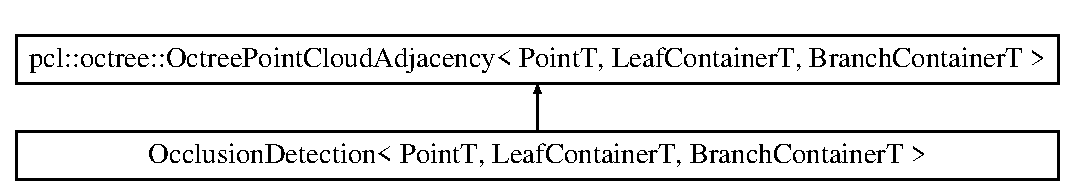
\includegraphics[height=2.000000cm]{classOcclusionDetection}
\end{center}
\end{figure}
\subsection*{Public Member Functions}
\begin{DoxyCompactItemize}
\item 
\hyperlink{classOcclusionDetection_acc151a65df0a4c19941c8af11c499deb}{Occlusion\+Detection} (const double resolution\+\_\+arg)
\item 
\hyperlink{classOcclusionDetection_ae4b87aa0e0cd1806dab5ceebf8eb1992}{$\sim$\+Occlusion\+Detection} ()
\item 
float \hyperlink{classOcclusionDetection_a7085e4d2d0e2d952f90fa366c73a12bc}{test\+For\+Occlusion2} (const PointT \&point\+\_\+arg, const pcl\+::\+Point\+X\+YZ \&camera\+\_\+pos)
\end{DoxyCompactItemize}
\subsection*{Private Attributes}
\begin{DoxyCompactItemize}
\item 
float \hyperlink{classOcclusionDetection_a1ae68b099e17672264520484de90d0c0}{resolution\+\_\+}
\end{DoxyCompactItemize}


\subsection{Constructor \& Destructor Documentation}
\mbox{\Hypertarget{classOcclusionDetection_acc151a65df0a4c19941c8af11c499deb}\label{classOcclusionDetection_acc151a65df0a4c19941c8af11c499deb}} 
\index{Occlusion\+Detection@{Occlusion\+Detection}!Occlusion\+Detection@{Occlusion\+Detection}}
\index{Occlusion\+Detection@{Occlusion\+Detection}!Occlusion\+Detection@{Occlusion\+Detection}}
\subsubsection{\texorpdfstring{Occlusion\+Detection()}{OcclusionDetection()}}
{\footnotesize\ttfamily template$<$typename PointT , typename Leaf\+ContainerT , typename Branch\+ContainerT $>$ \\
\hyperlink{classOcclusionDetection}{Occlusion\+Detection}$<$ PointT, Leaf\+ContainerT, Branch\+ContainerT $>$\+::\hyperlink{classOcclusionDetection}{Occlusion\+Detection} (\begin{DoxyParamCaption}\item[{const double}]{resolution\+\_\+arg }\end{DoxyParamCaption})}

\mbox{\Hypertarget{classOcclusionDetection_ae4b87aa0e0cd1806dab5ceebf8eb1992}\label{classOcclusionDetection_ae4b87aa0e0cd1806dab5ceebf8eb1992}} 
\index{Occlusion\+Detection@{Occlusion\+Detection}!````~Occlusion\+Detection@{$\sim$\+Occlusion\+Detection}}
\index{````~Occlusion\+Detection@{$\sim$\+Occlusion\+Detection}!Occlusion\+Detection@{Occlusion\+Detection}}
\subsubsection{\texorpdfstring{$\sim$\+Occlusion\+Detection()}{~OcclusionDetection()}}
{\footnotesize\ttfamily template$<$typename PointT , typename Leaf\+ContainerT  = Octree\+Point\+Cloud\+Adjacency\+Container $<$\+Point\+T$>$, typename Branch\+ContainerT  = Octree\+Container\+Empty$>$ \\
\hyperlink{classOcclusionDetection}{Occlusion\+Detection}$<$ PointT, Leaf\+ContainerT, Branch\+ContainerT $>$\+::$\sim$\hyperlink{classOcclusionDetection}{Occlusion\+Detection} (\begin{DoxyParamCaption}{ }\end{DoxyParamCaption})\hspace{0.3cm}{\ttfamily [inline]}}



\subsection{Member Function Documentation}
\mbox{\Hypertarget{classOcclusionDetection_a7085e4d2d0e2d952f90fa366c73a12bc}\label{classOcclusionDetection_a7085e4d2d0e2d952f90fa366c73a12bc}} 
\index{Occlusion\+Detection@{Occlusion\+Detection}!test\+For\+Occlusion2@{test\+For\+Occlusion2}}
\index{test\+For\+Occlusion2@{test\+For\+Occlusion2}!Occlusion\+Detection@{Occlusion\+Detection}}
\subsubsection{\texorpdfstring{test\+For\+Occlusion2()}{testForOcclusion2()}}
{\footnotesize\ttfamily template$<$typename PointT , typename Leaf\+ContainerT  = Octree\+Point\+Cloud\+Adjacency\+Container $<$\+Point\+T$>$, typename Branch\+ContainerT  = Octree\+Container\+Empty$>$ \\
float \hyperlink{classOcclusionDetection}{Occlusion\+Detection}$<$ PointT, Leaf\+ContainerT, Branch\+ContainerT $>$\+::test\+For\+Occlusion2 (\begin{DoxyParamCaption}\item[{const PointT \&}]{point\+\_\+arg,  }\item[{const pcl\+::\+Point\+X\+YZ \&}]{camera\+\_\+pos }\end{DoxyParamCaption})\hspace{0.3cm}{\ttfamily [inline]}}



\subsection{Member Data Documentation}
\mbox{\Hypertarget{classOcclusionDetection_a1ae68b099e17672264520484de90d0c0}\label{classOcclusionDetection_a1ae68b099e17672264520484de90d0c0}} 
\index{Occlusion\+Detection@{Occlusion\+Detection}!resolution\+\_\+@{resolution\+\_\+}}
\index{resolution\+\_\+@{resolution\+\_\+}!Occlusion\+Detection@{Occlusion\+Detection}}
\subsubsection{\texorpdfstring{resolution\+\_\+}{resolution\_}}
{\footnotesize\ttfamily template$<$typename PointT , typename Leaf\+ContainerT  = Octree\+Point\+Cloud\+Adjacency\+Container $<$\+Point\+T$>$, typename Branch\+ContainerT  = Octree\+Container\+Empty$>$ \\
float \hyperlink{classOcclusionDetection}{Occlusion\+Detection}$<$ PointT, Leaf\+ContainerT, Branch\+ContainerT $>$\+::resolution\+\_\+\hspace{0.3cm}{\ttfamily [private]}}



The documentation for this class was generated from the following file\+:\begin{DoxyCompactItemize}
\item 
src/\hyperlink{dynamic__obstacle__tracking_8cpp}{dynamic\+\_\+obstacle\+\_\+tracking.\+cpp}\end{DoxyCompactItemize}

\hypertarget{classmot_1_1tracked__object}{}\section{mot.\+tracked\+\_\+object Class Reference}
\label{classmot_1_1tracked__object}\index{mot.\+tracked\+\_\+object@{mot.\+tracked\+\_\+object}}


caution\#\#\#\#\#\# current tracking will be in xz plane only, z will be managed once convex hull part is figured out  


\subsection*{Public Member Functions}
\begin{DoxyCompactItemize}
\item 
def \hyperlink{classmot_1_1tracked__object_a15a1a975124c8c8a87232063ea9c8f37}{\+\_\+\+\_\+init\+\_\+\+\_\+} (self, \hyperlink{classmot_1_1tracked__object_ac78ee1daddcff29c0edbef88e4370ffa}{x}=0.\+0, \hyperlink{classmot_1_1tracked__object_abd3e436fb18ba75bbdcef0142ffc5dee}{y}=0.\+0, \hyperlink{classmot_1_1tracked__object_a557c82a367e7932c8ee09d6173ef8a4c}{z}=0.\+0, \hyperlink{classmot_1_1tracked__object_a35a31c9e6f822eae9ff5ca5f72678687}{is\+\_\+active}=False, \hyperlink{classmot_1_1tracked__object_a67774c920ad68d87e2ec5c9c24c6fc41}{is\+\_\+dead}=False, \hyperlink{classmot_1_1tracked__object_a28e39b4317941f7dbd7d5c9b1586a414}{youth}=0, \hyperlink{classmot_1_1tracked__object_a83c8c4e2de30738f82b230237ae7ef78}{strikes}=0, dt=0.\+16)
\item 
def \hyperlink{classmot_1_1tracked__object_acc90761003e14a1270e517f7b9b356da}{update\+\_\+matrices} (self, dt)
\item 
def \hyperlink{classmot_1_1tracked__object_ad5c025903cca465d22650a01e70dac44}{activate} (self)
\item 
def \hyperlink{classmot_1_1tracked__object_a4e36f1b91847d6d64890026eb7f51924}{deactivate} (self)
\item 
def \hyperlink{classmot_1_1tracked__object_a222ae20784de687532efc54632299b4a}{dead} (self)
\item 
def \hyperlink{classmot_1_1tracked__object_a85d7a4f4ea22ab10a426b344cc5fa827}{\+\_\+\+\_\+str\+\_\+\+\_\+} (self)
\end{DoxyCompactItemize}
\subsection*{Public Attributes}
\begin{DoxyCompactItemize}
\item 
\hyperlink{classmot_1_1tracked__object_a2e1c170f5477636531ae08ae12d0b17f}{id}
\item 
\hyperlink{classmot_1_1tracked__object_ac78ee1daddcff29c0edbef88e4370ffa}{x}
\item 
\hyperlink{classmot_1_1tracked__object_abd3e436fb18ba75bbdcef0142ffc5dee}{y}
\item 
\hyperlink{classmot_1_1tracked__object_a557c82a367e7932c8ee09d6173ef8a4c}{z}
\item 
\hyperlink{classmot_1_1tracked__object_a35a31c9e6f822eae9ff5ca5f72678687}{is\+\_\+active}
\item 
\hyperlink{classmot_1_1tracked__object_a67774c920ad68d87e2ec5c9c24c6fc41}{is\+\_\+dead}
\item 
\hyperlink{classmot_1_1tracked__object_a28e39b4317941f7dbd7d5c9b1586a414}{youth}
\item 
\hyperlink{classmot_1_1tracked__object_a83c8c4e2de30738f82b230237ae7ef78}{strikes}
\item 
\hyperlink{classmot_1_1tracked__object_a0f664cb6dc1c47a03245a3db2d6a3d20}{color}
\item 
\hyperlink{classmot_1_1tracked__object_a9fbaab65f9687617dbda8a32f11f729e}{kf}
\end{DoxyCompactItemize}


\subsection{Detailed Description}
caution\#\#\#\#\#\# current tracking will be in xz plane only, z will be managed once convex hull part is figured out 

\begin{DoxyVerb}Class to make individual tracked objects. More attributes can be added as detection algorithms evolve \end{DoxyVerb}
 

\subsection{Constructor \& Destructor Documentation}
\mbox{\Hypertarget{classmot_1_1tracked__object_a15a1a975124c8c8a87232063ea9c8f37}\label{classmot_1_1tracked__object_a15a1a975124c8c8a87232063ea9c8f37}} 
\index{mot\+::tracked\+\_\+object@{mot\+::tracked\+\_\+object}!\+\_\+\+\_\+init\+\_\+\+\_\+@{\+\_\+\+\_\+init\+\_\+\+\_\+}}
\index{\+\_\+\+\_\+init\+\_\+\+\_\+@{\+\_\+\+\_\+init\+\_\+\+\_\+}!mot\+::tracked\+\_\+object@{mot\+::tracked\+\_\+object}}
\subsubsection{\texorpdfstring{\+\_\+\+\_\+init\+\_\+\+\_\+()}{\_\_init\_\_()}}
{\footnotesize\ttfamily def mot.\+tracked\+\_\+object.\+\_\+\+\_\+init\+\_\+\+\_\+ (\begin{DoxyParamCaption}\item[{}]{self,  }\item[{}]{x = {\ttfamily 0.0},  }\item[{}]{y = {\ttfamily 0.0},  }\item[{}]{z = {\ttfamily 0.0},  }\item[{}]{is\+\_\+active = {\ttfamily False},  }\item[{}]{is\+\_\+dead = {\ttfamily False},  }\item[{}]{youth = {\ttfamily 0},  }\item[{}]{strikes = {\ttfamily 0},  }\item[{}]{dt = {\ttfamily 0.16} }\end{DoxyParamCaption})}

\begin{DoxyVerb}x and yare coordinates of the the obstacles in the plane they are moving. is_active determines if a marker is to be published for this object.
Youth variable is used to track the number of frames a new object appears, this is to filter out transient noise. Strikes calculate how long the object was not tracked.
\end{DoxyVerb}
 

\subsection{Member Function Documentation}
\mbox{\Hypertarget{classmot_1_1tracked__object_a85d7a4f4ea22ab10a426b344cc5fa827}\label{classmot_1_1tracked__object_a85d7a4f4ea22ab10a426b344cc5fa827}} 
\index{mot\+::tracked\+\_\+object@{mot\+::tracked\+\_\+object}!\+\_\+\+\_\+str\+\_\+\+\_\+@{\+\_\+\+\_\+str\+\_\+\+\_\+}}
\index{\+\_\+\+\_\+str\+\_\+\+\_\+@{\+\_\+\+\_\+str\+\_\+\+\_\+}!mot\+::tracked\+\_\+object@{mot\+::tracked\+\_\+object}}
\subsubsection{\texorpdfstring{\+\_\+\+\_\+str\+\_\+\+\_\+()}{\_\_str\_\_()}}
{\footnotesize\ttfamily def mot.\+tracked\+\_\+object.\+\_\+\+\_\+str\+\_\+\+\_\+ (\begin{DoxyParamCaption}\item[{}]{self }\end{DoxyParamCaption})}

\mbox{\Hypertarget{classmot_1_1tracked__object_ad5c025903cca465d22650a01e70dac44}\label{classmot_1_1tracked__object_ad5c025903cca465d22650a01e70dac44}} 
\index{mot\+::tracked\+\_\+object@{mot\+::tracked\+\_\+object}!activate@{activate}}
\index{activate@{activate}!mot\+::tracked\+\_\+object@{mot\+::tracked\+\_\+object}}
\subsubsection{\texorpdfstring{activate()}{activate()}}
{\footnotesize\ttfamily def mot.\+tracked\+\_\+object.\+activate (\begin{DoxyParamCaption}\item[{}]{self }\end{DoxyParamCaption})}

\mbox{\Hypertarget{classmot_1_1tracked__object_a4e36f1b91847d6d64890026eb7f51924}\label{classmot_1_1tracked__object_a4e36f1b91847d6d64890026eb7f51924}} 
\index{mot\+::tracked\+\_\+object@{mot\+::tracked\+\_\+object}!deactivate@{deactivate}}
\index{deactivate@{deactivate}!mot\+::tracked\+\_\+object@{mot\+::tracked\+\_\+object}}
\subsubsection{\texorpdfstring{deactivate()}{deactivate()}}
{\footnotesize\ttfamily def mot.\+tracked\+\_\+object.\+deactivate (\begin{DoxyParamCaption}\item[{}]{self }\end{DoxyParamCaption})}

\mbox{\Hypertarget{classmot_1_1tracked__object_a222ae20784de687532efc54632299b4a}\label{classmot_1_1tracked__object_a222ae20784de687532efc54632299b4a}} 
\index{mot\+::tracked\+\_\+object@{mot\+::tracked\+\_\+object}!dead@{dead}}
\index{dead@{dead}!mot\+::tracked\+\_\+object@{mot\+::tracked\+\_\+object}}
\subsubsection{\texorpdfstring{dead()}{dead()}}
{\footnotesize\ttfamily def mot.\+tracked\+\_\+object.\+dead (\begin{DoxyParamCaption}\item[{}]{self }\end{DoxyParamCaption})}

\mbox{\Hypertarget{classmot_1_1tracked__object_acc90761003e14a1270e517f7b9b356da}\label{classmot_1_1tracked__object_acc90761003e14a1270e517f7b9b356da}} 
\index{mot\+::tracked\+\_\+object@{mot\+::tracked\+\_\+object}!update\+\_\+matrices@{update\+\_\+matrices}}
\index{update\+\_\+matrices@{update\+\_\+matrices}!mot\+::tracked\+\_\+object@{mot\+::tracked\+\_\+object}}
\subsubsection{\texorpdfstring{update\+\_\+matrices()}{update\_matrices()}}
{\footnotesize\ttfamily def mot.\+tracked\+\_\+object.\+update\+\_\+matrices (\begin{DoxyParamCaption}\item[{}]{self,  }\item[{}]{dt }\end{DoxyParamCaption})}



\subsection{Member Data Documentation}
\mbox{\Hypertarget{classmot_1_1tracked__object_a0f664cb6dc1c47a03245a3db2d6a3d20}\label{classmot_1_1tracked__object_a0f664cb6dc1c47a03245a3db2d6a3d20}} 
\index{mot\+::tracked\+\_\+object@{mot\+::tracked\+\_\+object}!color@{color}}
\index{color@{color}!mot\+::tracked\+\_\+object@{mot\+::tracked\+\_\+object}}
\subsubsection{\texorpdfstring{color}{color}}
{\footnotesize\ttfamily mot.\+tracked\+\_\+object.\+color}

\mbox{\Hypertarget{classmot_1_1tracked__object_a2e1c170f5477636531ae08ae12d0b17f}\label{classmot_1_1tracked__object_a2e1c170f5477636531ae08ae12d0b17f}} 
\index{mot\+::tracked\+\_\+object@{mot\+::tracked\+\_\+object}!id@{id}}
\index{id@{id}!mot\+::tracked\+\_\+object@{mot\+::tracked\+\_\+object}}
\subsubsection{\texorpdfstring{id}{id}}
{\footnotesize\ttfamily mot.\+tracked\+\_\+object.\+id}

\mbox{\Hypertarget{classmot_1_1tracked__object_a35a31c9e6f822eae9ff5ca5f72678687}\label{classmot_1_1tracked__object_a35a31c9e6f822eae9ff5ca5f72678687}} 
\index{mot\+::tracked\+\_\+object@{mot\+::tracked\+\_\+object}!is\+\_\+active@{is\+\_\+active}}
\index{is\+\_\+active@{is\+\_\+active}!mot\+::tracked\+\_\+object@{mot\+::tracked\+\_\+object}}
\subsubsection{\texorpdfstring{is\+\_\+active}{is\_active}}
{\footnotesize\ttfamily mot.\+tracked\+\_\+object.\+is\+\_\+active}

\mbox{\Hypertarget{classmot_1_1tracked__object_a67774c920ad68d87e2ec5c9c24c6fc41}\label{classmot_1_1tracked__object_a67774c920ad68d87e2ec5c9c24c6fc41}} 
\index{mot\+::tracked\+\_\+object@{mot\+::tracked\+\_\+object}!is\+\_\+dead@{is\+\_\+dead}}
\index{is\+\_\+dead@{is\+\_\+dead}!mot\+::tracked\+\_\+object@{mot\+::tracked\+\_\+object}}
\subsubsection{\texorpdfstring{is\+\_\+dead}{is\_dead}}
{\footnotesize\ttfamily mot.\+tracked\+\_\+object.\+is\+\_\+dead}

\mbox{\Hypertarget{classmot_1_1tracked__object_a9fbaab65f9687617dbda8a32f11f729e}\label{classmot_1_1tracked__object_a9fbaab65f9687617dbda8a32f11f729e}} 
\index{mot\+::tracked\+\_\+object@{mot\+::tracked\+\_\+object}!kf@{kf}}
\index{kf@{kf}!mot\+::tracked\+\_\+object@{mot\+::tracked\+\_\+object}}
\subsubsection{\texorpdfstring{kf}{kf}}
{\footnotesize\ttfamily mot.\+tracked\+\_\+object.\+kf}

\mbox{\Hypertarget{classmot_1_1tracked__object_a83c8c4e2de30738f82b230237ae7ef78}\label{classmot_1_1tracked__object_a83c8c4e2de30738f82b230237ae7ef78}} 
\index{mot\+::tracked\+\_\+object@{mot\+::tracked\+\_\+object}!strikes@{strikes}}
\index{strikes@{strikes}!mot\+::tracked\+\_\+object@{mot\+::tracked\+\_\+object}}
\subsubsection{\texorpdfstring{strikes}{strikes}}
{\footnotesize\ttfamily mot.\+tracked\+\_\+object.\+strikes}

\mbox{\Hypertarget{classmot_1_1tracked__object_ac78ee1daddcff29c0edbef88e4370ffa}\label{classmot_1_1tracked__object_ac78ee1daddcff29c0edbef88e4370ffa}} 
\index{mot\+::tracked\+\_\+object@{mot\+::tracked\+\_\+object}!x@{x}}
\index{x@{x}!mot\+::tracked\+\_\+object@{mot\+::tracked\+\_\+object}}
\subsubsection{\texorpdfstring{x}{x}}
{\footnotesize\ttfamily mot.\+tracked\+\_\+object.\+x}

\mbox{\Hypertarget{classmot_1_1tracked__object_abd3e436fb18ba75bbdcef0142ffc5dee}\label{classmot_1_1tracked__object_abd3e436fb18ba75bbdcef0142ffc5dee}} 
\index{mot\+::tracked\+\_\+object@{mot\+::tracked\+\_\+object}!y@{y}}
\index{y@{y}!mot\+::tracked\+\_\+object@{mot\+::tracked\+\_\+object}}
\subsubsection{\texorpdfstring{y}{y}}
{\footnotesize\ttfamily mot.\+tracked\+\_\+object.\+y}

\mbox{\Hypertarget{classmot_1_1tracked__object_a28e39b4317941f7dbd7d5c9b1586a414}\label{classmot_1_1tracked__object_a28e39b4317941f7dbd7d5c9b1586a414}} 
\index{mot\+::tracked\+\_\+object@{mot\+::tracked\+\_\+object}!youth@{youth}}
\index{youth@{youth}!mot\+::tracked\+\_\+object@{mot\+::tracked\+\_\+object}}
\subsubsection{\texorpdfstring{youth}{youth}}
{\footnotesize\ttfamily mot.\+tracked\+\_\+object.\+youth}

\mbox{\Hypertarget{classmot_1_1tracked__object_a557c82a367e7932c8ee09d6173ef8a4c}\label{classmot_1_1tracked__object_a557c82a367e7932c8ee09d6173ef8a4c}} 
\index{mot\+::tracked\+\_\+object@{mot\+::tracked\+\_\+object}!z@{z}}
\index{z@{z}!mot\+::tracked\+\_\+object@{mot\+::tracked\+\_\+object}}
\subsubsection{\texorpdfstring{z}{z}}
{\footnotesize\ttfamily mot.\+tracked\+\_\+object.\+z}



The documentation for this class was generated from the following file\+:\begin{DoxyCompactItemize}
\item 
scripts/\hyperlink{mot_8py}{mot.\+py}\end{DoxyCompactItemize}

\hypertarget{classVelodyne}{}\section{Velodyne Class Reference}
\label{classVelodyne}\index{Velodyne@{Velodyne}}
Inheritance diagram for Velodyne\+:\begin{figure}[H]
\begin{center}
\leavevmode
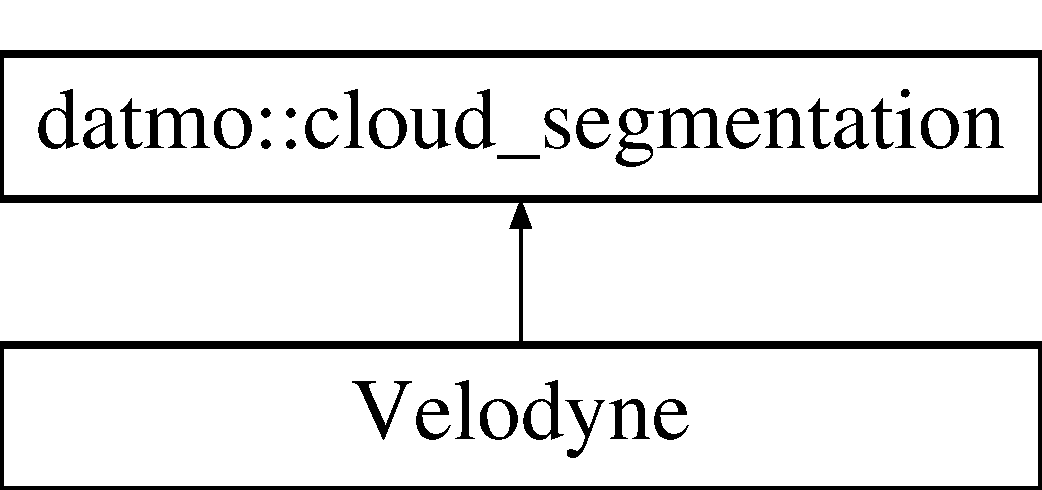
\includegraphics[height=2.000000cm]{classVelodyne}
\end{center}
\end{figure}
\subsection*{Public Member Functions}
\begin{DoxyCompactItemize}
\item 
\hyperlink{classVelodyne_aea299a13d4d1de508599627f52cf958c}{Velodyne} ()
\item 
\hyperlink{classVelodyne_a4e6654c8d061f82a062af273d75bbede}{$\sim$\+Velodyne} ()
\item 
void \hyperlink{classVelodyne_acc1ec7c74ba56c6330d94481960459a1}{init} (ros\+::\+Node\+Handle \&nh, ros\+::\+Node\+Handle \&private\+\_\+nh)
\end{DoxyCompactItemize}
\subsection*{Protected Attributes}
\begin{DoxyCompactItemize}
\item 
dynamic\+\_\+reconfigure\+::\+Server$<$ dynamic\+\_\+obstacle\+\_\+tracking\+::velodyne\+Config $>$ \hyperlink{classVelodyne_ae3c8869e849b22dad034e50dfbfccc1d}{server}
\item 
dynamic\+\_\+reconfigure\+::\+Server$<$ dynamic\+\_\+obstacle\+\_\+tracking\+::velodyne\+Config $>$\+::Callback\+Type \hyperlink{classVelodyne_aba02cf51ec41e7289dc2df2511d421ce}{cb\+\_\+type}
\end{DoxyCompactItemize}
\subsection*{Private Member Functions}
\begin{DoxyCompactItemize}
\item 
void \hyperlink{classVelodyne_a1a2fc80abf53b67444e0d6cc6916271a}{dynamic\+\_\+reconfigure\+\_\+cb} (dynamic\+\_\+obstacle\+\_\+tracking\+::velodyne\+Config \&config, uint32\+\_\+t level)
\end{DoxyCompactItemize}


\subsection{Constructor \& Destructor Documentation}
\mbox{\Hypertarget{classVelodyne_aea299a13d4d1de508599627f52cf958c}\label{classVelodyne_aea299a13d4d1de508599627f52cf958c}} 
\index{Velodyne@{Velodyne}!Velodyne@{Velodyne}}
\index{Velodyne@{Velodyne}!Velodyne@{Velodyne}}
\subsubsection{\texorpdfstring{Velodyne()}{Velodyne()}}
{\footnotesize\ttfamily Velodyne\+::\+Velodyne (\begin{DoxyParamCaption}{ }\end{DoxyParamCaption})}

\mbox{\Hypertarget{classVelodyne_a4e6654c8d061f82a062af273d75bbede}\label{classVelodyne_a4e6654c8d061f82a062af273d75bbede}} 
\index{Velodyne@{Velodyne}!````~Velodyne@{$\sim$\+Velodyne}}
\index{````~Velodyne@{$\sim$\+Velodyne}!Velodyne@{Velodyne}}
\subsubsection{\texorpdfstring{$\sim$\+Velodyne()}{~Velodyne()}}
{\footnotesize\ttfamily Velodyne\+::$\sim$\+Velodyne (\begin{DoxyParamCaption}{ }\end{DoxyParamCaption})}



\subsection{Member Function Documentation}
\mbox{\Hypertarget{classVelodyne_a1a2fc80abf53b67444e0d6cc6916271a}\label{classVelodyne_a1a2fc80abf53b67444e0d6cc6916271a}} 
\index{Velodyne@{Velodyne}!dynamic\+\_\+reconfigure\+\_\+cb@{dynamic\+\_\+reconfigure\+\_\+cb}}
\index{dynamic\+\_\+reconfigure\+\_\+cb@{dynamic\+\_\+reconfigure\+\_\+cb}!Velodyne@{Velodyne}}
\subsubsection{\texorpdfstring{dynamic\+\_\+reconfigure\+\_\+cb()}{dynamic\_reconfigure\_cb()}}
{\footnotesize\ttfamily void Velodyne\+::dynamic\+\_\+reconfigure\+\_\+cb (\begin{DoxyParamCaption}\item[{dynamic\+\_\+obstacle\+\_\+tracking\+::velodyne\+Config \&}]{config,  }\item[{uint32\+\_\+t}]{level }\end{DoxyParamCaption})\hspace{0.3cm}{\ttfamily [private]}}

\mbox{\Hypertarget{classVelodyne_acc1ec7c74ba56c6330d94481960459a1}\label{classVelodyne_acc1ec7c74ba56c6330d94481960459a1}} 
\index{Velodyne@{Velodyne}!init@{init}}
\index{init@{init}!Velodyne@{Velodyne}}
\subsubsection{\texorpdfstring{init()}{init()}}
{\footnotesize\ttfamily void Velodyne\+::init (\begin{DoxyParamCaption}\item[{ros\+::\+Node\+Handle \&}]{nh,  }\item[{ros\+::\+Node\+Handle \&}]{private\+\_\+nh }\end{DoxyParamCaption})}

$<$ minimum value of x

$<$ maximum value of x 

\subsection{Member Data Documentation}
\mbox{\Hypertarget{classVelodyne_aba02cf51ec41e7289dc2df2511d421ce}\label{classVelodyne_aba02cf51ec41e7289dc2df2511d421ce}} 
\index{Velodyne@{Velodyne}!cb\+\_\+type@{cb\+\_\+type}}
\index{cb\+\_\+type@{cb\+\_\+type}!Velodyne@{Velodyne}}
\subsubsection{\texorpdfstring{cb\+\_\+type}{cb\_type}}
{\footnotesize\ttfamily dynamic\+\_\+reconfigure\+::\+Server$<$dynamic\+\_\+obstacle\+\_\+tracking\+::velodyne\+Config$>$\+::Callback\+Type Velodyne\+::cb\+\_\+type\hspace{0.3cm}{\ttfamily [protected]}}

\mbox{\Hypertarget{classVelodyne_ae3c8869e849b22dad034e50dfbfccc1d}\label{classVelodyne_ae3c8869e849b22dad034e50dfbfccc1d}} 
\index{Velodyne@{Velodyne}!server@{server}}
\index{server@{server}!Velodyne@{Velodyne}}
\subsubsection{\texorpdfstring{server}{server}}
{\footnotesize\ttfamily dynamic\+\_\+reconfigure\+::\+Server$<$dynamic\+\_\+obstacle\+\_\+tracking\+::velodyne\+Config$>$ Velodyne\+::server\hspace{0.3cm}{\ttfamily [protected]}}



The documentation for this class was generated from the following file\+:\begin{DoxyCompactItemize}
\item 
src/\hyperlink{velodyne__node_8cpp}{velodyne\+\_\+node.\+cpp}\end{DoxyCompactItemize}

\hypertarget{classZR300}{}\section{Z\+R300 Class Reference}
\label{classZR300}\index{Z\+R300@{Z\+R300}}
Inheritance diagram for Z\+R300\+:\begin{figure}[H]
\begin{center}
\leavevmode
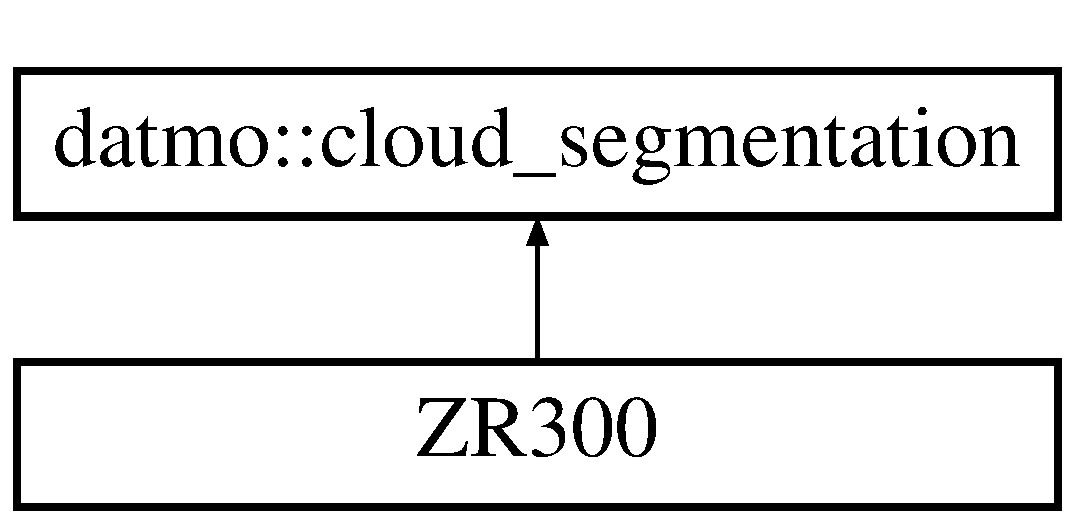
\includegraphics[height=2.000000cm]{classZR300}
\end{center}
\end{figure}
\subsection*{Public Member Functions}
\begin{DoxyCompactItemize}
\item 
\hyperlink{classZR300_a63a89a9de2af2d6d30ecf039b64c48a3}{Z\+R300} ()
\item 
\hyperlink{classZR300_af9ecd118c1a33dd2da78693de057c8b5}{$\sim$\+Z\+R300} ()
\item 
void \hyperlink{classZR300_aaecbf7e995d17a699c3305bc60dc547d}{init} (ros\+::\+Node\+Handle \&nh, ros\+::\+Node\+Handle \&private\+\_\+nh)
\end{DoxyCompactItemize}
\subsection*{Protected Attributes}
\begin{DoxyCompactItemize}
\item 
dynamic\+\_\+reconfigure\+::\+Server$<$ dynamic\+\_\+obstacle\+\_\+tracking\+::zr300\+Config $>$ \hyperlink{classZR300_afe2acfe42f2153ef3a488367ffdfcca0}{server}
\item 
dynamic\+\_\+reconfigure\+::\+Server$<$ dynamic\+\_\+obstacle\+\_\+tracking\+::zr300\+Config $>$\+::Callback\+Type \hyperlink{classZR300_ad68d353c780b751ba511b67f9b475b01}{cb\+\_\+type}
\end{DoxyCompactItemize}
\subsection*{Private Member Functions}
\begin{DoxyCompactItemize}
\item 
void \hyperlink{classZR300_a562f13a7e98d8b7b58818194d5aa142e}{dynamic\+\_\+reconfigure\+\_\+cb} (dynamic\+\_\+obstacle\+\_\+tracking\+::zr300\+Config \&config, uint32\+\_\+t level)
\end{DoxyCompactItemize}


\subsection{Constructor \& Destructor Documentation}
\mbox{\Hypertarget{classZR300_a63a89a9de2af2d6d30ecf039b64c48a3}\label{classZR300_a63a89a9de2af2d6d30ecf039b64c48a3}} 
\index{Z\+R300@{Z\+R300}!Z\+R300@{Z\+R300}}
\index{Z\+R300@{Z\+R300}!Z\+R300@{Z\+R300}}
\subsubsection{\texorpdfstring{Z\+R300()}{ZR300()}}
{\footnotesize\ttfamily Z\+R300\+::\+Z\+R300 (\begin{DoxyParamCaption}{ }\end{DoxyParamCaption})}

\mbox{\Hypertarget{classZR300_af9ecd118c1a33dd2da78693de057c8b5}\label{classZR300_af9ecd118c1a33dd2da78693de057c8b5}} 
\index{Z\+R300@{Z\+R300}!````~Z\+R300@{$\sim$\+Z\+R300}}
\index{````~Z\+R300@{$\sim$\+Z\+R300}!Z\+R300@{Z\+R300}}
\subsubsection{\texorpdfstring{$\sim$\+Z\+R300()}{~ZR300()}}
{\footnotesize\ttfamily Z\+R300\+::$\sim$\+Z\+R300 (\begin{DoxyParamCaption}{ }\end{DoxyParamCaption})}



\subsection{Member Function Documentation}
\mbox{\Hypertarget{classZR300_a562f13a7e98d8b7b58818194d5aa142e}\label{classZR300_a562f13a7e98d8b7b58818194d5aa142e}} 
\index{Z\+R300@{Z\+R300}!dynamic\+\_\+reconfigure\+\_\+cb@{dynamic\+\_\+reconfigure\+\_\+cb}}
\index{dynamic\+\_\+reconfigure\+\_\+cb@{dynamic\+\_\+reconfigure\+\_\+cb}!Z\+R300@{Z\+R300}}
\subsubsection{\texorpdfstring{dynamic\+\_\+reconfigure\+\_\+cb()}{dynamic\_reconfigure\_cb()}}
{\footnotesize\ttfamily void Z\+R300\+::dynamic\+\_\+reconfigure\+\_\+cb (\begin{DoxyParamCaption}\item[{dynamic\+\_\+obstacle\+\_\+tracking\+::zr300\+Config \&}]{config,  }\item[{uint32\+\_\+t}]{level }\end{DoxyParamCaption})\hspace{0.3cm}{\ttfamily [private]}}

\mbox{\Hypertarget{classZR300_aaecbf7e995d17a699c3305bc60dc547d}\label{classZR300_aaecbf7e995d17a699c3305bc60dc547d}} 
\index{Z\+R300@{Z\+R300}!init@{init}}
\index{init@{init}!Z\+R300@{Z\+R300}}
\subsubsection{\texorpdfstring{init()}{init()}}
{\footnotesize\ttfamily void Z\+R300\+::init (\begin{DoxyParamCaption}\item[{ros\+::\+Node\+Handle \&}]{nh,  }\item[{ros\+::\+Node\+Handle \&}]{private\+\_\+nh }\end{DoxyParamCaption})}



\subsection{Member Data Documentation}
\mbox{\Hypertarget{classZR300_ad68d353c780b751ba511b67f9b475b01}\label{classZR300_ad68d353c780b751ba511b67f9b475b01}} 
\index{Z\+R300@{Z\+R300}!cb\+\_\+type@{cb\+\_\+type}}
\index{cb\+\_\+type@{cb\+\_\+type}!Z\+R300@{Z\+R300}}
\subsubsection{\texorpdfstring{cb\+\_\+type}{cb\_type}}
{\footnotesize\ttfamily dynamic\+\_\+reconfigure\+::\+Server$<$dynamic\+\_\+obstacle\+\_\+tracking\+::zr300\+Config$>$\+::Callback\+Type Z\+R300\+::cb\+\_\+type\hspace{0.3cm}{\ttfamily [protected]}}

\mbox{\Hypertarget{classZR300_afe2acfe42f2153ef3a488367ffdfcca0}\label{classZR300_afe2acfe42f2153ef3a488367ffdfcca0}} 
\index{Z\+R300@{Z\+R300}!server@{server}}
\index{server@{server}!Z\+R300@{Z\+R300}}
\subsubsection{\texorpdfstring{server}{server}}
{\footnotesize\ttfamily dynamic\+\_\+reconfigure\+::\+Server$<$dynamic\+\_\+obstacle\+\_\+tracking\+::zr300\+Config$>$ Z\+R300\+::server\hspace{0.3cm}{\ttfamily [protected]}}



The documentation for this class was generated from the following file\+:\begin{DoxyCompactItemize}
\item 
src/\hyperlink{zr300__node_8cpp}{zr300\+\_\+node.\+cpp}\end{DoxyCompactItemize}

\chapter{File Documentation}
\hypertarget{dynamic__obstacle__tracking_8hpp}{}\section{include/dynamic\+\_\+obstacle\+\_\+tracking/dynamic\+\_\+obstacle\+\_\+tracking.hpp File Reference}
\label{dynamic__obstacle__tracking_8hpp}\index{include/dynamic\+\_\+obstacle\+\_\+tracking/dynamic\+\_\+obstacle\+\_\+tracking.\+hpp@{include/dynamic\+\_\+obstacle\+\_\+tracking/dynamic\+\_\+obstacle\+\_\+tracking.\+hpp}}
{\ttfamily \#include $<$ros/ros.\+h$>$}\newline
{\ttfamily \#include $<$visualization\+\_\+msgs/\+Marker.\+h$>$}\newline
{\ttfamily \#include $<$visualization\+\_\+msgs/\+Marker\+Array.\+h$>$}\newline
{\ttfamily \#include $<$sensor\+\_\+msgs/\+Point\+Cloud2.\+h$>$}\newline
{\ttfamily \#include $<$nav\+\_\+msgs/\+Odometry.\+h$>$}\newline
{\ttfamily \#include $<$geometry\+\_\+msgs/\+Pose\+Array.\+h$>$}\newline
{\ttfamily \#include $<$geometry\+\_\+msgs/\+Pose.\+h$>$}\newline
{\ttfamily \#include $<$dynamic\+\_\+reconfigure/server.\+h$>$}\newline
{\ttfamily \#include $<$pcl\+\_\+conversions/pcl\+\_\+conversions.\+h$>$}\newline
{\ttfamily \#include $<$pcl/point\+\_\+cloud.\+h$>$}\newline
{\ttfamily \#include $<$pcl/point\+\_\+types.\+h$>$}\newline
{\ttfamily \#include $<$pcl/common/transforms.\+h$>$}\newline
{\ttfamily \#include $<$pcl/common/common.\+h$>$}\newline
{\ttfamily \#include $<$Eigen/\+Dense$>$}\newline
{\ttfamily \#include $<$Eigen/\+Geometry$>$}\newline
{\ttfamily \#include $<$math.\+h$>$}\newline
{\ttfamily \#include $<$tf/\+Linear\+Math/\+Matrix3x3.\+h$>$}\newline
{\ttfamily \#include $<$tf/transform\+\_\+datatypes.\+h$>$}\newline
{\ttfamily \#include $<$tf/transform\+\_\+listener.\+h$>$}\newline
{\ttfamily \#include $<$tf/transform\+\_\+broadcaster.\+h$>$}\newline
{\ttfamily \#include \char`\"{}tf\+\_\+conversions/tf\+\_\+eigen.\+h\char`\"{}}\newline
{\ttfamily \#include $<$pcl/filters/passthrough.\+h$>$}\newline
{\ttfamily \#include $<$pcl/registration/icp.\+h$>$}\newline
{\ttfamily \#include $<$pcl/filters/voxel\+\_\+grid.\+h$>$}\newline
{\ttfamily \#include $<$pcl/filters/approximate\+\_\+voxel\+\_\+grid.\+h$>$}\newline
{\ttfamily \#include $<$pcl/filters/statistical\+\_\+outlier\+\_\+removal.\+h$>$}\newline
{\ttfamily \#include $<$pcl/features/normal\+\_\+3d.\+h$>$}\newline
{\ttfamily \#include $<$pcl/kdtree/kdtree.\+h$>$}\newline
{\ttfamily \#include $<$pcl/segmentation/extract\+\_\+clusters.\+h$>$}\newline
{\ttfamily \#include $<$pcl/octree/octree\+\_\+impl.\+h$>$}\newline
{\ttfamily \#include $<$pcl/octree/octree.\+h$>$}\newline
{\ttfamily \#include $<$pcl/octree/octree\+\_\+pointcloud\+\_\+adjacency.\+h$>$}\newline
{\ttfamily \#include $<$pcl/sample\+\_\+consensus/method\+\_\+types.\+h$>$}\newline
{\ttfamily \#include $<$pcl/sample\+\_\+consensus/model\+\_\+types.\+h$>$}\newline
{\ttfamily \#include $<$pcl/segmentation/sac\+\_\+segmentation.\+h$>$}\newline
{\ttfamily \#include $<$pcl/\+Model\+Coefficients.\+h$>$}\newline
{\ttfamily \#include $<$pcl/filters/extract\+\_\+indices.\+h$>$}\newline
{\ttfamily \#include $<$ctime$>$}\newline
\subsection*{Classes}
\begin{DoxyCompactItemize}
\item 
struct \hyperlink{structdatmo_1_1Float3}{datmo\+::\+Float3}
\item 
class \hyperlink{classdatmo_1_1cloud__segmentation}{datmo\+::cloud\+\_\+segmentation}
\end{DoxyCompactItemize}
\subsection*{Namespaces}
\begin{DoxyCompactItemize}
\item 
 \hyperlink{namespacedatmo}{datmo}
\end{DoxyCompactItemize}
\subsection*{Macros}
\begin{DoxyCompactItemize}
\item 
\#define \hyperlink{dynamic__obstacle__tracking_8hpp_a598a3330b3c21701223ee0ca14316eca}{PI}~3.\+14159265
\item 
\#define \hyperlink{dynamic__obstacle__tracking_8hpp_ad41630f833e920c1ffa34722f45a8e77}{S\+QR}(a)~((a)$\ast$(a))
\end{DoxyCompactItemize}


\subsection{Macro Definition Documentation}
\mbox{\Hypertarget{dynamic__obstacle__tracking_8hpp_a598a3330b3c21701223ee0ca14316eca}\label{dynamic__obstacle__tracking_8hpp_a598a3330b3c21701223ee0ca14316eca}} 
\index{dynamic\+\_\+obstacle\+\_\+tracking.\+hpp@{dynamic\+\_\+obstacle\+\_\+tracking.\+hpp}!PI@{PI}}
\index{PI@{PI}!dynamic\+\_\+obstacle\+\_\+tracking.\+hpp@{dynamic\+\_\+obstacle\+\_\+tracking.\+hpp}}
\subsubsection{\texorpdfstring{PI}{PI}}
{\footnotesize\ttfamily \#define PI~3.\+14159265}

\mbox{\Hypertarget{dynamic__obstacle__tracking_8hpp_ad41630f833e920c1ffa34722f45a8e77}\label{dynamic__obstacle__tracking_8hpp_ad41630f833e920c1ffa34722f45a8e77}} 
\index{dynamic\+\_\+obstacle\+\_\+tracking.\+hpp@{dynamic\+\_\+obstacle\+\_\+tracking.\+hpp}!S\+QR@{S\+QR}}
\index{S\+QR@{S\+QR}!dynamic\+\_\+obstacle\+\_\+tracking.\+hpp@{dynamic\+\_\+obstacle\+\_\+tracking.\+hpp}}
\subsubsection{\texorpdfstring{S\+QR}{SQR}}
{\footnotesize\ttfamily \#define S\+QR(\begin{DoxyParamCaption}\item[{}]{a }\end{DoxyParamCaption})~((a)$\ast$(a))}


\hypertarget{mot_8py}{}\section{scripts/mot.py File Reference}
\label{mot_8py}\index{scripts/mot.\+py@{scripts/mot.\+py}}
\subsection*{Classes}
\begin{DoxyCompactItemize}
\item 
class \hyperlink{classmot_1_1tracked__object}{mot.\+tracked\+\_\+object}
\begin{DoxyCompactList}\small\item\em caution\#\#\#\#\#\# current tracking will be in xz plane only, z will be managed once convex hull part is figured out \end{DoxyCompactList}\item 
class \hyperlink{classmot_1_1Mot}{mot.\+Mot}
\end{DoxyCompactItemize}
\subsection*{Namespaces}
\begin{DoxyCompactItemize}
\item 
 \hyperlink{namespacemot}{mot}
\end{DoxyCompactItemize}
\subsection*{Functions}
\begin{DoxyCompactItemize}
\item 
def \hyperlink{namespacemot_a0aeef71e241eafce8fb5d73cfe5ef0e7}{mot.\+main} ()
\end{DoxyCompactItemize}
\subsection*{Variables}
\begin{DoxyCompactItemize}
\item 
list \hyperlink{namespacemot_a175bf1670619de28a5c8277715c2aee5}{mot.\+color\+\_\+pallete} = \mbox{[}Color\+R\+G\+BA(0.\+8941176470588236, 0.\+10196078431372549, 0.\+10980392156862745, 0.\+3), Color\+R\+G\+BA(0.\+21568627450980393, 0.\+49411764705882355, 0.\+7215686274509804, 0.\+3), Color\+R\+G\+BA(0.\+30196078431372547, 0.\+6862745098039216, 0.\+2901960784313726, 0.\+3), Color\+R\+G\+BA(0.\+596078431372549, 0.\+3058823529411765, 0.\+6392156862745098, 0.\+3), Color\+R\+G\+BA(1.\+0, 0.\+4980392156862745, 0.\+0, 0.\+3), Color\+R\+G\+BA(1.\+0, 1.\+0, 0.\+2, 0.\+3), Color\+R\+G\+BA(0.\+6509803921568628, 0.\+33725490196078434, 0.\+1568627450980392, 0.\+3), Color\+R\+G\+BA(0.\+9686274509803922, 0.\+5058823529411764, 0.\+7490196078431373, 0.\+3), Color\+R\+G\+BA(0.\+6, 0.\+6, 0.\+6, 0.\+3)\mbox{]}
\end{DoxyCompactItemize}

\hypertarget{dynamic__obstacle__tracking_8cpp}{}\section{src/dynamic\+\_\+obstacle\+\_\+tracking.cpp File Reference}
\label{dynamic__obstacle__tracking_8cpp}\index{src/dynamic\+\_\+obstacle\+\_\+tracking.\+cpp@{src/dynamic\+\_\+obstacle\+\_\+tracking.\+cpp}}
{\ttfamily \#include $<$dynamic\+\_\+obstacle\+\_\+tracking/dynamic\+\_\+obstacle\+\_\+tracking.\+hpp$>$}\newline
\subsection*{Classes}
\begin{DoxyCompactItemize}
\item 
class \hyperlink{classOcclusionDetection}{Occlusion\+Detection$<$ Point\+T, Leaf\+Container\+T, Branch\+Container\+T $>$}
\end{DoxyCompactItemize}

\hypertarget{velodyne__node_8cpp}{}\section{src/velodyne\+\_\+node.cpp File Reference}
\label{velodyne__node_8cpp}\index{src/velodyne\+\_\+node.\+cpp@{src/velodyne\+\_\+node.\+cpp}}
{\ttfamily \#include $<$ros/ros.\+h$>$}\newline
{\ttfamily \#include $<$dynamic\+\_\+obstacle\+\_\+tracking/dynamic\+\_\+obstacle\+\_\+tracking.\+hpp$>$}\newline
{\ttfamily \#include $<$dynamic\+\_\+obstacle\+\_\+tracking/velodyne\+Config.\+h$>$}\newline
\subsection*{Classes}
\begin{DoxyCompactItemize}
\item 
class \hyperlink{classSensor}{Sensor}
\end{DoxyCompactItemize}
\subsection*{Functions}
\begin{DoxyCompactItemize}
\item 
int \hyperlink{velodyne__node_8cpp_a3c04138a5bfe5d72780bb7e82a18e627}{main} (int argc, char $\ast$$\ast$argv)
\end{DoxyCompactItemize}


\subsection{Function Documentation}
\mbox{\Hypertarget{velodyne__node_8cpp_a3c04138a5bfe5d72780bb7e82a18e627}\label{velodyne__node_8cpp_a3c04138a5bfe5d72780bb7e82a18e627}} 
\index{velodyne\+\_\+node.\+cpp@{velodyne\+\_\+node.\+cpp}!main@{main}}
\index{main@{main}!velodyne\+\_\+node.\+cpp@{velodyne\+\_\+node.\+cpp}}
\subsubsection{\texorpdfstring{main()}{main()}}
{\footnotesize\ttfamily int main (\begin{DoxyParamCaption}\item[{int}]{argc,  }\item[{char $\ast$$\ast$}]{argv }\end{DoxyParamCaption})}


\hypertarget{zr300__node_8cpp}{}\section{src/zr300\+\_\+node.cpp File Reference}
\label{zr300__node_8cpp}\index{src/zr300\+\_\+node.\+cpp@{src/zr300\+\_\+node.\+cpp}}
{\ttfamily \#include $<$ros/ros.\+h$>$}\newline
{\ttfamily \#include $<$dynamic\+\_\+obstacle\+\_\+tracking/dynamic\+\_\+obstacle\+\_\+tracking.\+hpp$>$}\newline
{\ttfamily \#include $<$dynamic\+\_\+obstacle\+\_\+tracking/zr300\+Config.\+h$>$}\newline
\subsection*{Classes}
\begin{DoxyCompactItemize}
\item 
class \hyperlink{classZR300}{Z\+R300}
\end{DoxyCompactItemize}
\subsection*{Functions}
\begin{DoxyCompactItemize}
\item 
int \hyperlink{zr300__node_8cpp_a3c04138a5bfe5d72780bb7e82a18e627}{main} (int argc, char $\ast$$\ast$argv)
\end{DoxyCompactItemize}


\subsection{Function Documentation}
\mbox{\Hypertarget{zr300__node_8cpp_a3c04138a5bfe5d72780bb7e82a18e627}\label{zr300__node_8cpp_a3c04138a5bfe5d72780bb7e82a18e627}} 
\index{zr300\+\_\+node.\+cpp@{zr300\+\_\+node.\+cpp}!main@{main}}
\index{main@{main}!zr300\+\_\+node.\+cpp@{zr300\+\_\+node.\+cpp}}
\subsubsection{\texorpdfstring{main()}{main()}}
{\footnotesize\ttfamily int main (\begin{DoxyParamCaption}\item[{int}]{argc,  }\item[{char $\ast$$\ast$}]{argv }\end{DoxyParamCaption})}


%--- End generated contents ---

% Index
\backmatter
\newpage
\phantomsection
\clearemptydoublepage
\addcontentsline{toc}{chapter}{Index}
\printindex

\end{document}
